\documentclass[aspectratio=149, xcolor=table]{beamer}
\usetheme[compress]{Szeged}
%\usefonttheme{serif}
\usecolortheme{dove}
\useinnertheme{rounded}
\setbeamersize{text margin left=5mm,text margin right=10mm}
\usefonttheme{serif}
\usepackage{graphicx}
\usepackage[italian]{babel}
\usepackage[utf8]{inputenc}
\usepackage{tabularx}
\usepackage{tikz}
\usepackage[absolute,overlay]{textpos} 
\usepackage{xcolor}
\usepackage{multicol}
\usepackage{dcolumn}
\definecolor{myGreen}{RGB}{54, 114, 89}
\definecolor{unipd}{RGB}{155, 0, 20}
\definecolor{sbj1}{HTML}{77AC30}
\definecolor{Max}{HTML}{EDB120}
\definecolor{sbj3}{HTML}{0072BD}
\definecolor{sbj4}{HTML}{1F78B4}
\definecolor{sbj5}{HTML}{33A02C}
\definecolor{Jane}{HTML}{E31A1C}
\definecolor{royalblue3}{RGB}{58,95,205}
\definecolor{Joe}{RGB}{100, 149, 237}
% Per il tema Montpellier
%\setbeamercolor{separation line}{bg=myGreen!20}
\setbeamercolor{separation line}{bg=black!20}
%\setbeamercolor{title in head/foot}{bg=white, fg=myGreen}
\setbeamercolor{title in head/foot}{bg=white, fg=black}
%\setbeamercolor{section in head/foot}{bg=white, fg=myGreen}
%\setbeamercolor{subsection in head/foot}{bg=white, fg=myGreen}
%\setbeamercolor{background canvas}{bg=white}
%\setbeamercolor{title}{fg=myGreen}
%\setbeamercolor{item}{fg =myGreen}
%\setbeamercolor{frametitle}{fg = myGreen}
%\setbeamercolor{section in toc}{fg=myGreen!80}
%\setbeamercolor{subsection in toc}{fg=black}
\setbeamerfont{section in toc}{series=\bfseries,size=\normalsize}
\setbeamerfont{frametitle}{series=\bfseries}
%\setbeamerfont{title}{family=\scshape}
%\setbeamercolor{frametitle}{fg=unipd}
%\setbeamercolor{section in head/foot}{bg=unipd, fg=white}
%\setbeamercolor{subsection in head/foot}{fg=unipd}
%\setbeamercolor{author in head/foot}{bg=unipd, fg=white}
%\setbeamercolor{title in head/foot}{fg=unipd}
%\setbeamercolor{date in head/foot}{fg=unipd}
 \setbeamercolor{block title}{fg=unipd}
%\setbeamercolor{block body}{bg=yellow!20, fg=black}
% definisce gli elementi da mettere sopra la figura 
% rectangles on figures 
\newcommand{\imagenode}[2][1]% [scale], filename
{   \node[above right,inner sep=0] (myimage) {\includegraphics[scale=#1]{#2}};
	\path (myimage.north east);
	\pgfgetlastxy{\myimagex}{\myimagey}
	\pgfmathsetmacro{\myimagewidth}{\myimagex/28.453}
	\pgfmathsetmacro{\myimageheight}{\myimagey/28.453}
}
\newcommand{\imagegrid}[4][help lines]% [options], steps, font, precision
{   \pgfkeys{/pgf/number format/.cd,fixed,precision=#4}
	\foreach \x in {0,...,#2}
	{   \draw[#1] (\x/#2*\myimagewidth,\myimageheight) -- (\x/#2*\myimagewidth,0) node[below] {#3\pgfmathparse{\x/#2}\pgfmathprintnumber{\pgfmathresult}};
		\draw[#1] (\myimagewidth,\x/#2*\myimageheight) -- (0,\x/#2*\myimageheight) node[left] {#3\pgfmathparse{\x/#2}\pgfmathprintnumber{\pgfmathresult}};
	}
}

\newcommand{\highlightbox}[8][densely dashed,thick]% [options], left, low, right, up, node options, node text, overlay spec
{   \only<#8>{\draw[#1] (#2*\myimagewidth, #3*\myimageheight) rectangle node[#6] {#7} (#4*\myimagewidth, #5*\myimageheight);}
}

\newcommand{\highlighttext}[8][densely dashed,thick]% [options], left, low, right, up, node options, node text, overlay spec
{   \only<#8>{\path[#1] (#2*\myimagewidth, #3*\myimageheight) rectangle node[#6] {#7} (#4*\myimagewidth, #5*\myimageheight);}
}
\newcolumntype{d}[1]{D{.}{.}{#1}}
\def\sym#1{\ifmmode^{#1}\else\(^{#1}\)\fi}

% tikz per la cfa 

\usetikzlibrary{shapes.geometric, arrows}
\tikzstyle{latent} = [ellipse, minimum width=2.5cm, minimum height=2cm,text centered, draw=black]
\tikzstyle{item} = [rectangle, rounded corners, minimum width=0.5cm, minimum height=1cm, text width =1.5cm, text centered, draw=black]
\tikzstyle{arrow} = [thick,->,>=stealth]

% allegedly, il codice che viene dopo permette di cambiare colore alle celle 

\makeatletter
\def\rowcolor{\noalign{\ifnum0=`}\fi\bmr@rowcolor}
\newcommand<>{\bmr@rowcolor}{%
	\alt#1%
	{\global\let\CT@do@color\CT@@do@color\@ifnextchar[\CT@rowa\CT@rowb}% 
	{\ifnum0=`{\fi}\@gooble@rowcolor}% 
}

\newcommand{\@gooble@rowcolor}[2][]{\@gooble@rowcolor@}
\newcommand{\@gooble@rowcolor@}[1][]{\@gooble@rowcolor@@}
\newcommand{\@gooble@rowcolor@@}[1][]{\ignorespaces}
\makeatother



\makeatletter
\def\cellcolor{{\ifnum0=`}\fi\bmr@cellcolor}
\newcommand<>{\bmr@cellcolor}{%
	\alt#1%
	{\global\let\CT@do@color\CT@@do@color\@ifnextchar[\CT@rowa\CT@rowb}% 
	{\ifnum0=`{\fi}\@gooble@cellcolor}% 
}

\newcommand{\@gooble@cellcolor}[2][]{\@gooble@cellcolor@}
\newcommand{\@gooble@cellcolor@}[1][]{\@gooble@cellcolor@@}
\newcommand{\@gooble@cellcolor@@}[1][]{\ignorespaces}
\makeatother

\AtBeginSection[]
{
	\begin{frame}
		\tableofcontents[currentsection, currentsubsection]
	\end{frame}
}

\AtBeginSubsection[]
{
	\begin{frame}
		\tableofcontents[currentsection, currentsubsection]
	\end{frame}
}


\title[Meaningfulness]{L'importanza di essere significante:\\ Un esempio basato sul test della Torre di Londra}
\author[Epifania et al.]{\textbf{Ottavia M. Epifania}, Luca Stefanutti, Pasquale Anselmi,  Andrea Brancaccio, Debora de Chiusole}
\institute [UniPd] {
	
\includegraphics[width=10mm]{unipd.png}\\ 
Dipartimento di Filosofia, Sociologia, Pedagogia e Psicologia Applicata,\\	Università di Padova}
	
	\date [Giornata 03] {%\vspace{0.6cm}\\
	La psicometria tra oggi e domani: \\ Sfide e nuovi orizzonti \\ \vspace{3mm}
		20 Giugno 2023}
\begin{document}
	
	\begin{frame}[plain]
		\maketitle
	\end{frame}

\section{Meaningfulness}


\begin{frame}
	
	The ratio between the measures of $a$ and $b$ is constant and independent of the measurement unit:
	\[
	\frac{\varphi(a)}{\varphi(b)} = \frac{\varphi'(a)}{\varphi'(b)},
	\]
	
	where $\varphi$ and $\varphi'$ are two different scales of measurement of the same variable.
	
	\pause
	\begin{block}{Meaningful comparisons}
		
		The comparison between \emph{a} and \emph{b} is meaningful if it is invariant under all the unit transformations. 
			
	\end{block}
	
	\pause
	\begin{block}{Beyond meaningful comparison}
		Given that there is a difference between $a$ and $b$, is this difference significant (or not) regardless of the scales of measurement?
	\end{block}
	\color{blue}
\end{frame}


\subsection*{Admissible and non-admissible transformations}

\begin{frame}
	\begin{columns}[T]
		\begin{column}{.30\linewidth}
		
		$\varphi (P) = [0, 1, 2, 3]$ 
		\end{column}
			\begin{column}{.30\linewidth}
		
		$\varphi' (P) = [0, 2, 4, 10]$ 
		\end{column}
		
		\onslide<3->
			\begin{column}{.30\linewidth}
	
	$\varepsilon (P) = [0, 2, 3]$ 
		\end{column}
	\end{columns}

\onslide<2->
	\vspace{3.5mm}
	\begin{minipage}{.7\linewidth}

			\scalebox{.8}{
			\begin{tabular}{l rrr rrr rrr}
				\multicolumn{10}{c}{$\varphi$} \\
				&	it01	&	it02	&	it03	&	it04	&	it05	&	it06	&	it07	&	it08	&	it09			\\
				\color{Joe}Joe\normalcolor	&	0	&	1	&	2	&	2	&	2	&	3	&	3	&	3	&	3			\\
				\color{Jane}Jane\normalcolor	&	0	&	2	&	2	&	2	&	3	&	3	&	3	&	3	&	3			\\
				\color{Max}Max\normalcolor	&	0	&	1	&	0	&	2	&	3	&	3	&	3	&	3	&	3			\\
				
				\multicolumn{10}{c}{$\varphi'$} \\
				%		&	it01	&	it02	&	it03	&	it04	&	it05	&	it06	&	it07	&	it08	&	it09			\\
				Joe	&	0	&	2	&	4	&	4	&	4	&	10	&	10	&	10	&	10			\\
				Jane	&	0	&	4	&	4	&	4	&	10	&	10	&	10	&	10	&	10			\\
				Max	&	0	&	2	&	0	&	4	&	10	&	10	&	10	&	10	&	10			\\
				\multicolumn{10}{c}{\onslide<4->$\epsilon$} \\
			%		&	it01	&	it02	&	it03	&	it04	&	it05	&	it06	&	it07	&	it08	&	it09			\\
			\onslide<4->Joe	&	\onslide<4->0	&	\onslide<4->2	&	\onslide<4->2	&	\onslide<4->2	&	\onslide<4->2	&	\onslide<4->3	&	\onslide<4->3	&	\onslide<4->3	&	\onslide<4->3			\\
			\onslide<4->Jane	&	\onslide<4->0	&	\onslide<4->2	&	\onslide<4->2	&	\onslide<4->2	&	\onslide<4->3	&	\onslide<4->3	&	\onslide<4->3	&	\onslide<4->3	&	\onslide<4->3			\\
			\onslide<4->Max	&	\onslide<4->0	&	\onslide<4->2	&	\onslide<4->0	&	\onslide<4->2	&	\onslide<4->3	&	\onslide<4->3	&	\onslide<4->3	&	\onslide<4->3	&	\onslide<4->3			\\
			
			\end{tabular}	
}
	\end{minipage}%
\begin{minipage}{.30\linewidth}
	\begin{columns}[T]
\onslide<2->
		\begin{column}{.30\linewidth}
			\centering
				\begin{tikzpicture}
				
				% Coordinates for the dots
				\coordinate (A) at (0, 0);
				\coordinate (B) at (0, 1);
				\coordinate (C) at (0, 2);
				
				% Drawing the vertical line
				\draw[thick] (0, 0) -- (0, 2);
				
				% Drawing the dots with labels
				\fill[Max] (A) circle (3pt) node[right] {18};
				\fill[Joe] (B) circle (3pt) node[right] {19};
				\fill[Jane] (C) circle (3pt) node[right] {21};
				
				% Adding the title
				\node at (0, 3) {\centering $\varphi$};
			\end{tikzpicture}
		
		\end{column}
		\begin{column}{.30\linewidth}
				\centering
			\begin{tikzpicture}
				
				% Coordinates for the dots
				\coordinate (A) at (0, 0);
				\coordinate (B) at (0, 1);
				\coordinate (C) at (0, 2);
				
				% Drawing the vertical line
				\draw[thick] (0, 0) -- (0, 2);
				
				% Drawing the dots with labels
				\fill[Joe] (A) circle (3pt) node[right] {54};
				\fill[Max] (B) circle (3pt) node[right] {56};
				\fill[Jane] (C) circle (3pt) node[right] {62};
				
				% Adding the title
				\node at (0, 3) {\centering $\varphi'$};
			\end{tikzpicture}
			
		\end{column}

		\begin{column}{.30\linewidth}
				\centering
				
			\begin{tikzpicture}
			
			% Coordinates for the dots
			\coordinate (A) at (0, 0);
			\coordinate (B) at (0, 1);
			\coordinate (C) at (0, 2);
			
			% Drawing the vertical line
			\draw[thick] (0, 0) -- (0, 2);
			
			% Drawing the dots with labels
			\fill[Max] (A) circle (3pt) node[right] {22};
			\fill[Joe] (B) circle (3pt) node[right] {23};
			\fill[Jane] (C) circle (3pt) node[right] {24};
			
			% Adding the title
			\node at (0, 3) {\centering $\varepsilon$};
		\end{tikzpicture}
			
		\end{column}
	\end{columns}
\end{minipage}
\end{frame}

%\begin{frame}
%	 \begin{figure}[h]
%	 	
%	 	\scalebox{.80}{
%	 		\begin{tikzpicture}
%	 			\draw[->,thick] (0,0) -- (12,0) node[right] {time (sec)};
%	 			\draw[thick] (0,-.1) node[below] {$0$} --(0,.1);
%	 			\draw[thick] (3.33,-.1) node[below] {$15$} --(3.33,.1);
%	 			\draw[thick] (5.55,-.1) node[below] {$25$} --(5.55,.1);	
%	 			\draw[thick] (6.66,-.1) node[below] {$30$} --(6.66,.1);	
%	 			\draw[thick] (10,-.1) node[below] {$45$} --(10,.1);	
%	 			%	\draw[thick] (10,-.1) node[below] {$60$} --(10,.1);	
%	 			\node at (1.7,.5) {$4$};
%	 			\node at (4.75,.5) {$3$};
%	 			\node at (6,.5) {$2$};
%	 			\node at (8.25,.5) {$1$};
%	 			\node at (10.5,.5) {$0$};
%	 			%	\node at (10.5,.5) {$0$};
%	 			\node at (-1,0) {\Large\color{unipd}$\varphi$};
%	 		\end{tikzpicture}
%	 		
%	 	}
%	 	
%	 \end{figure}
%	 
%	 \begin{figure}
%	 	\scalebox{.80}{
%	 		\begin{tikzpicture}
%	 			\draw[->, thick] (0,0) -- (12,0) node[right] {time (sec)};
%	 			\draw[thick] (0,-.1) node[below] {$0$} --(0,.1);
%	 			\draw[thick] (4.44,-.1) node[below] {$20$} --(4.44,.1);
%	 			\draw[thick] (6.66,-.1) node[below] {$30$} --(6.66,.1);	
%	 			\draw[thick] (7.77,-.1) node[below] {$35$} --(7.77,.1);	
%	 			\draw[thick] (11.11,-.1) node[below] {$50$} --(11.11,.1);	
%	 			\node at (2.22,.5) {$4$};
%	 			\node at (5.55,.5) {$3$};
%	 			\node at (7,.5) {$2$};
%	 			\node at (9.25,.5) {$1$};
%	 			\node at (11.5,.5) {$0$};
%	 			\node at (-1,0) {\Large\color{royalblue3}$\varphi'$};
%	 		\end{tikzpicture}
%	 	}
%	 	
%	 \end{figure}
%	 
%	 
%	 \onslide<2->
%	 \begin{table}
%	 	\begin{tabular}{cccc ccc cc}
%	 		\hline
%	 		
%	 		
%	 		Item	&	$t_A$	&	$t_B$	&	&	$\varphi_A$	&	$\varphi_B$	&	&	$\varphi_A'$	&	$\varphi_B'$	\\\hline
%	 		1	&	14	&	14	&	&	4	&	4	&	&	4	&	4	\\
%	 		2	&	26	&	19	&	&	2	&	3	&	&	3	&	4	\\
%	 		3	&	31	&	33	&	&	1	&	1	&	&	3	&	2	\\
%	 		4	&	46	&	18	&	&	0	&	3	&	&	1	&	4	\\
%	 		5	&	17	&	46	&	&	4	&	0	&	&	3	&	1	\\
%	 		\hline
%	 		Sum scores: & & & & 11 & 11 & & 14 & 15 \\
%	 		
%	 		\hline
%	 		
%	 	\end{tabular}
%	 \end{table}		
%	 \visible<3> {
%	 	\begin{tikzpicture}[overlay]
%	 		\draw[unipd,ultra thick,rounded corners] (6.7,0) rectangle (8.5,4);
%	 	\end{tikzpicture}
%	 }   
%	 
%	 \visible<4> {
%	 	\begin{tikzpicture}[overlay]
%	 		\draw[royalblue3,ultra thick,rounded corners] (9,0.5) rectangle (11,4.5);
%	 	\end{tikzpicture}
%	 }   
%	 
%\end{frame}

\section{The case in point}
\subsection{Tower of London}
\begin{frame}
	
	\begin{columns}
		\column{0.45\textwidth}
		\begin{center}
			\begin{tikzpicture}[scale=1.2]
				\node (start) [mark=diamond,inner sep = 0pt, minimum size = 4pt] (23) at (  -1.5,  3.5*1.73) {
					\begin{tikzpicture}[scale=.6]
						\draw[draw=black!20,fill=black!20] (0,5) rectangle (6,5.3);
						\draw[draw=black!20,fill=black!20] (0.85,5) rectangle (1.15,8.5);
						\draw[draw=black!20,fill=black!20] (2.85,5) rectangle (3.15,7.5);
						\draw[draw=black!20,fill=black!20] (4.85,5) rectangle (5.15,6.5);
						\draw[fill=red] (1,5.8) circle (15pt);
						\draw[fill=yellow] (5,5.8) circle (15pt);
						\draw[fill= blue] (3,5.8) circle (15pt);
					\end{tikzpicture}
				};
			\end{tikzpicture}\\
			Starting configuration
		\end{center}
		\column{0.45\textwidth}
		\begin{center}
			\begin{tikzpicture}[scale=1.2]
				\node (goal) [mark=diamond,inner sep = 0pt, minimum size = 4pt] (23) at (  -1.5,  3.5*1.73) {
					\begin{tikzpicture}[scale=.6]
						\draw[draw=black!20,fill=black!20] (0,5) rectangle (6,5.3);
						\draw[draw=black!20,fill=black!20] (0.85,5) rectangle (1.15,8.5);
						\draw[draw=black!20,fill=black!20] (2.85,5) rectangle (3.15,7.5);
						\draw[draw=black!20,fill=black!20] (4.85,5) rectangle (5.15,6.5);
						\draw[fill=yellow] (1,5.8) circle (15pt);
						\draw[fill=red] (1,6.85) circle (15pt);
						\draw[fill=blue] (3,5.8) circle (15pt);
					\end{tikzpicture}
				};
				
			\end{tikzpicture}\\
			Goal configuration 
		\end{center}
	\end{columns}

	\vspace{3mm}
	
	Problem complexity influenced by: 
	
	\begin{itemize}
		\item Number of moves
		\item Number of alternative paths
		\item Hierarchy of the starting/goal configuration
	\end{itemize}
	
	

	

\end{frame}



\subsection*{The Tower of London Test (ToL Test)}
\begin{frame}
	
	
	
	\begin{columns}[T]
		\column{0.45\textwidth}
		
		\begin{center}
			\small
			\begin{itemize}
				\item 12 problems    
				\vspace{.2cm}
				\item Same starting configuration
				\vspace{.2cm}
				\item More than one attempt per item 
			\end{itemize}
			
			\vspace{.3cm}
			\begin{tikzpicture}[scale=1.2]
				\node[mark=diamond,inner sep = 0pt, minimum size = 4pt] (23) at (  -1.5,  3.5*1.73) {
					\begin{tikzpicture}[scale=.4]
						\draw[draw=black!20,fill=black!20] (0,5) rectangle (6,5.3);
						\draw[draw=black!20,fill=black!20] (0.85,5) rectangle (1.15,8.5);
						\draw[draw=black!20,fill=black!20] (2.85,5) rectangle (3.15,7.5);
						\draw[draw=black!20,fill=black!20] (4.85,5) rectangle (5.15,6.5);
						\draw[fill=yellow] (1,5.8) circle (15pt);
						\draw[fill=red] (1,6.85) circle (15pt);
						\draw[fill=blue] (3,5.8) circle (15pt);
					\end{tikzpicture}
				};
			\end{tikzpicture}
		\end{center}
		
		\column{0.45\textwidth}
		\vspace{- .5cm}
		\begin{center}    
			\scriptsize
			
			\scalebox{.80}{
				\begin{tabular}{ccc}
				\hline
				Problem	&	Minimum moves	&	Alternative paths	\\
				\hline
				Example	&	2	&	1	\\
				1	&	2	&	1	\\
				2	&	2	&	1	\\
				3	&	3	&	2	\\
				4	&	3	&	1	\\
				5	&	4	&	2	\\
				6	&	4	&	1	\\
				7	&	4	&	1	\\
				8	&	4	&	1	\\
				9	&	5	&	2	\\
				10	&	5	&	1	\\
				11	&	5	&	1	\\
				12	&	5	&	2	\\
				\hline
			\end{tabular}
			}

		
		\end{center}
	\end{columns}
\end{frame}

\subsection[Attempt-based SMs]{Attempt-based scoring methods}

\begin{frame}
		\centering
		\scalebox{.75}{
			\begin{tabular}{|cllllc}
				%	\multicolumn{1}{c}{}	& \multicolumn{4}{c}{Score assigned to problems solved at: } &  \\	
				\hline
				Scoring system &  \multicolumn{1}{|c|}{First attempt} &  \multicolumn{1}{|c|}{Second attempt} &  \multicolumn{1}{|c|}{Third attempt} &  \multicolumn{1}{|c|}{Fourth on} & \multicolumn{1}{|c|}{Total sum score} \\ \cline{1-6}\hline
				KR &  \multicolumn{1}{|c|}{\cellcolor{green!20}{3}}  &\multicolumn{1}{|c|}{\cellcolor{yellow!20}{2}}&\multicolumn{1}{|c|}{\cellcolor{orange!30}1}& \multicolumn{1}{|c|}{\cellcolor{red!50}0} & \multicolumn{1}{|c|}{\cellcolor{white}0 -- 36}\\\cline{1-6}\hline
				SH1 &  \multicolumn{1}{|c|}{\cellcolor{green!20}1}& \multicolumn{3}{|c|}{\cellcolor{red!50}0} & \multicolumn{1}{|c|}{\cellcolor{white}0 -- 12} \\\hline
			

			\end{tabular}
		}

	\centering

\vspace{5mm}

\begin{overprint}
	\onslide<2>
		\scalebox{.75}{
		\begin{tabular}{|cllllc}
			%	\multicolumn{1}{c}{}	& \multicolumn{4}{c}{Score assigned to problems solved at: } &  \\	
			\hline
			Scoring system &  \multicolumn{1}{|c|}{First attempt} &  \multicolumn{1}{|c|}{Second attempt} &  \multicolumn{1}{|c|}{Third attempt} &  \multicolumn{1}{|c|}{Fourth on} & \multicolumn{1}{|c|}{Total sum score} \\\cline{1-6}\hline
			P1 &  \multicolumn{1}{|c|}{\cellcolor{green!20}3}& \multicolumn{2}{|c|}{\cellcolor{orange!30}2} & \multicolumn{1}{|c|}{\cellcolor{red!50}0}& \multicolumn{1}{|c|}{\cellcolor{white}0 -- 36}\\\cline{1-6}\hline
			P1$'$ &  \multicolumn{1}{|c|}{\cellcolor{green!20}3}& \multicolumn{2}{|c|}{\cellcolor{orange!30}1} & \multicolumn{1}{|c|}{\cellcolor{red!50}0} & \multicolumn{1}{|c|}{\cellcolor{white}0 -- 36}\\
			\hline
		\end{tabular}
	}
	\onslide<3>
		\scalebox{.75}{
		\begin{tabular}{|cllllc}
			%	\multicolumn{1}{c}{}	& \multicolumn{4}{c}{Score assigned to problems solved at: } &  \\	
			\hline
			Scoring system &  \multicolumn{1}{|c|}{First attempt} &  \multicolumn{1}{|c|}{Second attempt} &  \multicolumn{1}{|c|}{Third attempt} &  \multicolumn{1}{|c|}{Fourth on} & \multicolumn{1}{|c|}{Total sum score} \\\cline{1-6}\hline
			P1 &  \multicolumn{1}{|c|}{\cellcolor{green!20}3}& \multicolumn{2}{|c|}{\cellcolor{orange!30}\textbf{2}} & \multicolumn{1}{|c|}{\cellcolor{red!50}0}& \multicolumn{1}{|c|}{\cellcolor{white}0 -- 36}\\\cline{1-6}\hline
			P1$'$ &  \multicolumn{1}{|c|}{\cellcolor{green!20}3}& \multicolumn{2}{|c|}{\cellcolor{orange!30}\textbf{1}} & \multicolumn{1}{|c|}{\cellcolor{red!50}0} & \multicolumn{1}{|c|}{\cellcolor{white}0 -- 36}\\
			\hline
		\end{tabular}
	}
\end{overprint}
	
	

\end{frame}

\subsection[Latency-based SMs]{Latency-based scoring methods}
\begin{frame}
	\scalebox{.8}{
	\begin{minipage}{.\linewidth}
		
		\begin{tikzpicture}
			\draw[->,thick] (0,0) -- (12,0) node[right] {time (sec)};
			\draw[thick] (0,-.1) node[below] {$0$} --(0,.1);
			\draw[thick] (2.5,-.1) node[below] {$15$} --(2.5,.1);	
			\draw[thick] (5,-.1) node[below] {$30$} --(5,.1);	
			\draw[thick] (10,-.1) node[below] {$60$} --(10,.1);	
			\node at (1.5,.5) {$3$};
			\node at (4,.5) {$2$};
			\node at (7.5,.5) {$1$};
			\node at (10.5,.5) {$0$};
			\node at (-1,0) {SH2};
		\end{tikzpicture}
		
	\end{minipage}
	}
		
		\scalebox{.80}{
		\begin{minipage}{.\linewidth}
			\begin{center}
				\begin{tikzpicture}
					\draw[->,thick] (0,0) -- (12,0) node[right] {time (sec)};
					\draw[thick] (0,-.1) node[below] {$0$} --(0,.1);
					\draw[thick] (1,-.1) node[below] {$6$} --(1,.1);
					\draw[thick] (1.67,-.1) node[below] {$10$} --(1.67,.1);	
					\draw[thick] (3.33,-.1) node[below] {$20$} --(3.33,.1);	
					\draw[thick] (6.65,-.1) node[below] {$40$} --(6.65,.1);	
					\draw[thick] (10,-.1) node[below] {$60$} --(10,.1);	
					\node at (.5,.5) {$9$};
					\node at (1.25,.5) {$8$};
					\node at (2.5,.5) {$7$};
					\node at (5.25,.5) {$6$};
					\node at (8,.5) {$5$};
					\node at (10.5,.5) {$0$};
					\node at (-1,0) {AN};
				\end{tikzpicture}
			\end{center}
		\end{minipage}
		
		}
		
		\onslide<2->
		\vspace{5mm}
	\scalebox{.80}{
		\begin{minipage}{.\linewidth}
		\begin{center}
			\begin{tikzpicture}
				\draw[->,thick] (0,0) -- (12,0) node[right] {time (sec)};
				\draw[thick] (0,-.1) node[below] {$0$} --(0,.1);
				\draw[thick] (1,-.1) node[below] {$6$} --(1,.1);
				\draw[thick] (1.67,-.1) node[below] {$10$} --(1.67,.1);	
				\draw[thick] (3.33,-.1) node[below] {$20$} --(3.33,.1);	
				\draw[thick] (6.65,-.1) node[below] {$40$} --(6.65,.1);	
				\draw[thick] (10,-.1) node[below] {$60$} --(10,.1);	
				\node at (.5,.5) {$25$};
				\node at (1.25,.5) {$18$};
				\node at (2.5,.5) {$17$};
				\node at (5.25,.5) {$16$};
				\node at (8,.5) {$15$};
				\node at (10.5,.5) {$0$};
				\node at (-1,0) {\emph{T}};
			\end{tikzpicture}
		\end{center}
		
	\end{minipage}
	}
	



\end{frame}

%
%\subsection{Scoring systems}
%
%\begin{frame}
%
%
%\centering
%\scalebox{.80}{
%
%\begin{tabular}{l c c c c}
%\hline
%Scoring & Attempts & Response times & Item score & Total score \\\hline
%\textcolor<2->{black!15}{Shallice 1} & \textcolor<2->{black!15}{$\checkmark$} & \textcolor<2->{black!15}{$\checkmark$} & \textcolor<2->{black!15}{0-1} & \textcolor<2->{black!15}{0-12} \\
% \cellcolor<2>{black!20}Shallice 2 & $\times$ & $\checkmark$ &0-3 & 0-36\\
% \cellcolor<2>{black!20}Anderson et al. & $\checkmark$ & $\checkmark$ & 0-9& 0-108 \\
%\textcolor<2->{black!15}{Kirkorian et al.} & \textcolor<2->{black!15}{$\checkmark$} & \textcolor<2->{black!15}{$\times$} & \textcolor<2->{black!15}{0-3}& \textcolor<2->{black!15}{0-36} \\\hline
%
%
%\end{tabular}
%}
%
%
%\vspace{-1.5mm}
%\onslide<2->
%\begin{columns}[T]
%	\begin{column}{.50\linewidth}
%		\begin{center}
%			Shallice 2 -- SH2
%		\end{center}
%		\small
%			 For each of the 12 items:
%			\bigskip
%			
%			\centering
%			\begin{tabular}{cc}
%				\hline
%				Assign & if time is\\
%				\hline
%				3 & $\leq 15$ s \\
%				2 & $15 \dashv 30$ s \\
%				1 & $30 \dashv 60$ s \\
%				0 & $>60$ s \\
%				\hline
%			\end{tabular}
%			\bigskip
%			
%	\end{column}
%	
%		\begin{column}{.50\linewidth}
%			\begin{center}
%			Anderson et al. -- AN
%		\end{center}
%		\small
%		\centering
%			 For each of the 12 items:
%				\bigskip			
%				
%			\begin{tabular}{cl}
%				\hline
%				Assign & if time is\\
%				\hline
%				9 & $\leq6$ s \\
%				8 & $6\dashv10$ s \\
%				7 & $11\dashv20$ s \\
%				6 & $21\dashv40$ s \\
%				5 & $41\dashv60$ s \\
%				0 & $>60$ s \\
%				\hline
%			\end{tabular}
%			\footnotesize \normalfont 
%			\flushleft
%			
%			Subtract the number of unsuccessful attempts
%	\end{column}
%\end{columns}
%\end{frame}


\section{Real data application}

\subsection{Individual differences}

\begin{frame}

		
	\begin{columns}[T]
		\begin{column}{.50\linewidth}
			\begin{center}
				\textbf{Monotonic relation}
			\end{center}
			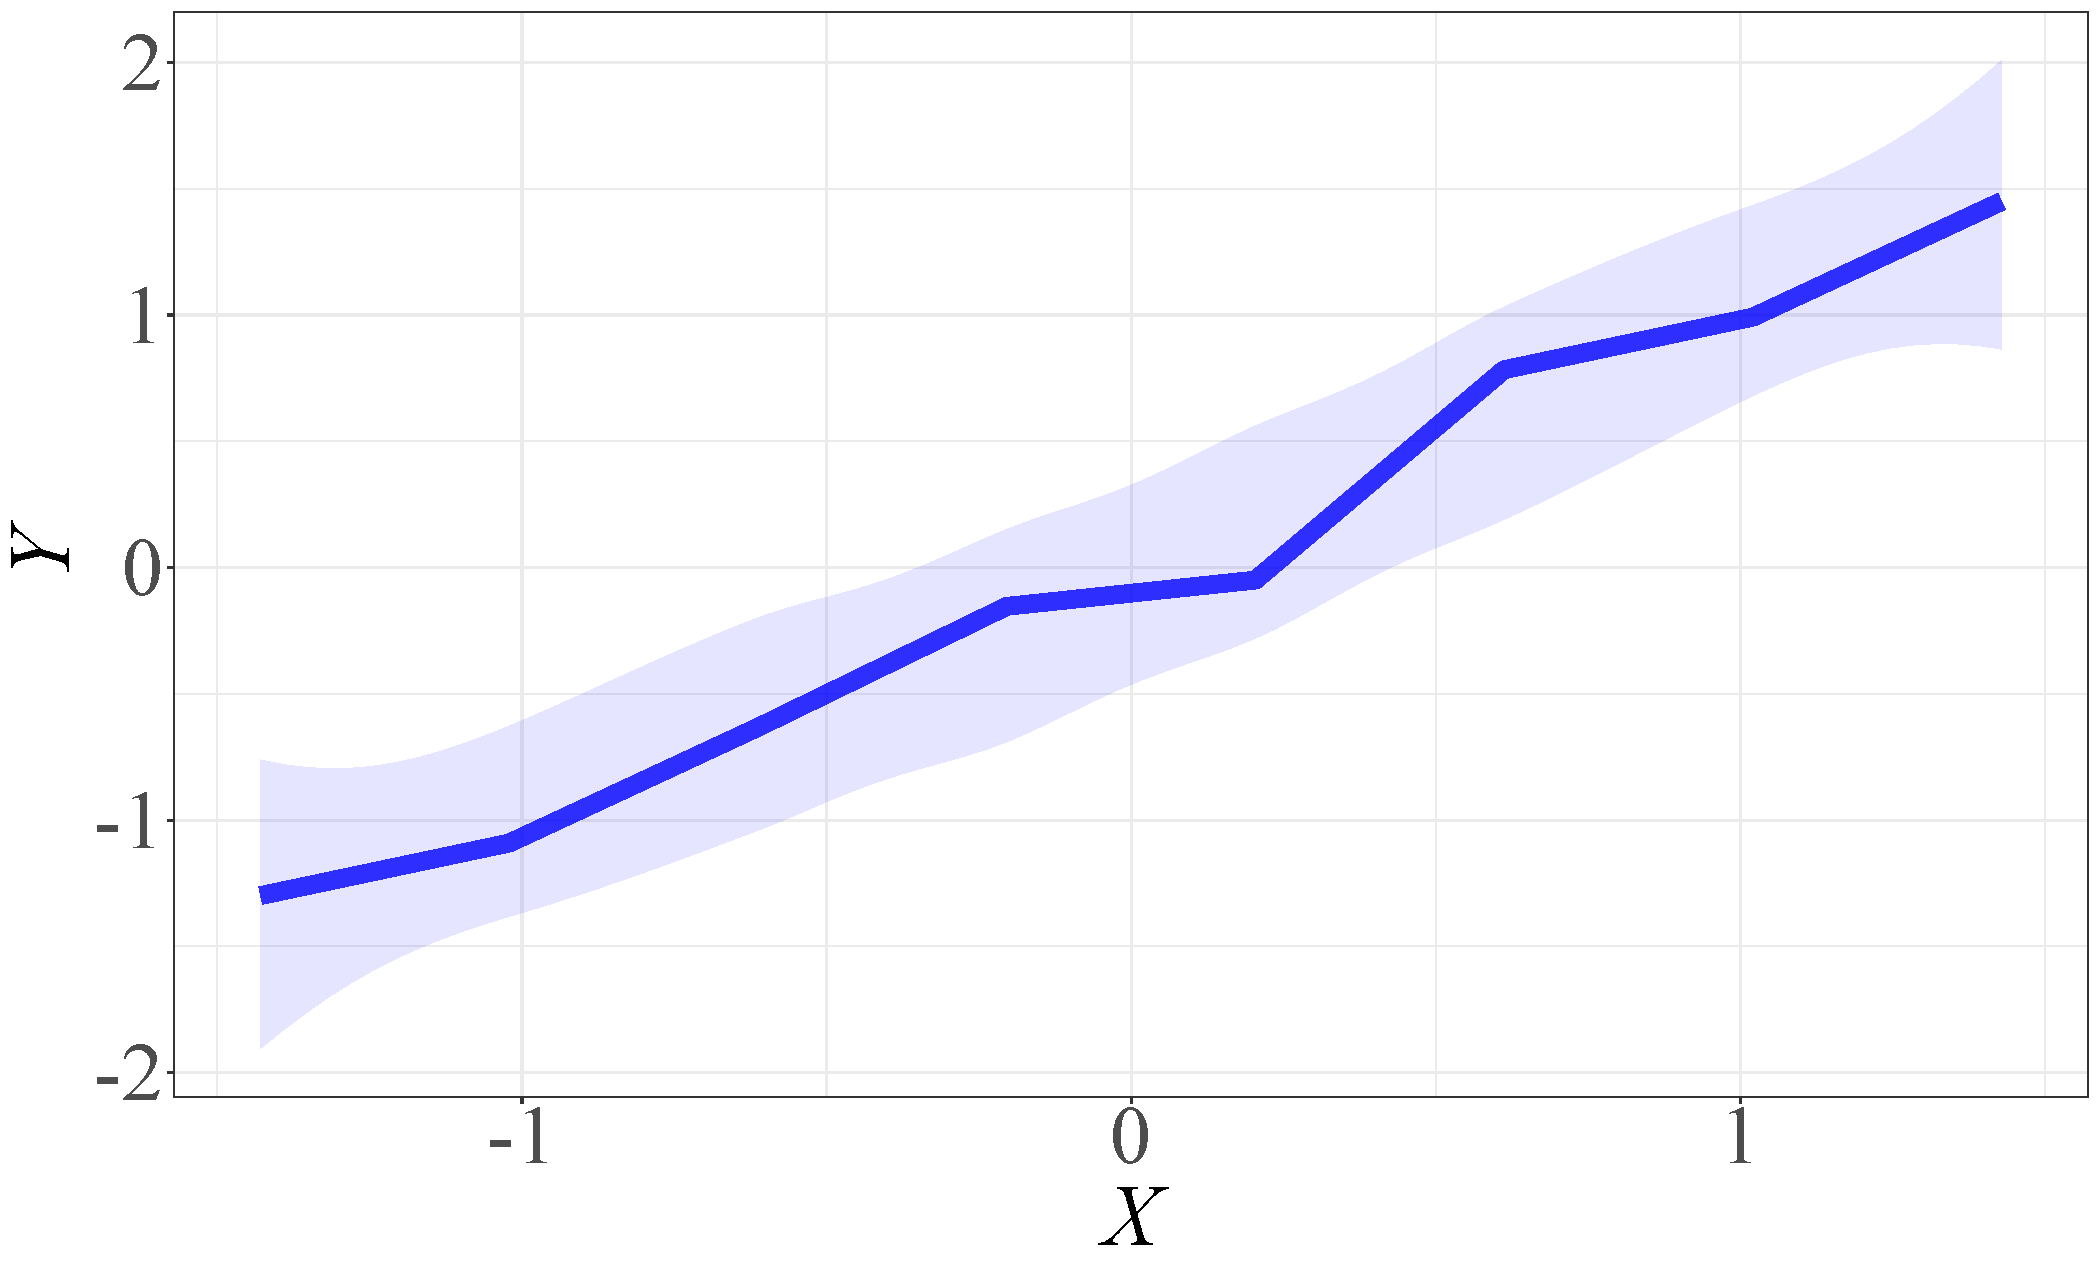
\includegraphics[width=\linewidth]{img/mono-relation}
		\end{column}
\onslide<2->
		\begin{column}{.50\linewidth}
			\begin{center}
				\textbf{Distances and inversions}
			\end{center}
			\begin{overprint}
				\centering
				\onslide<2>
					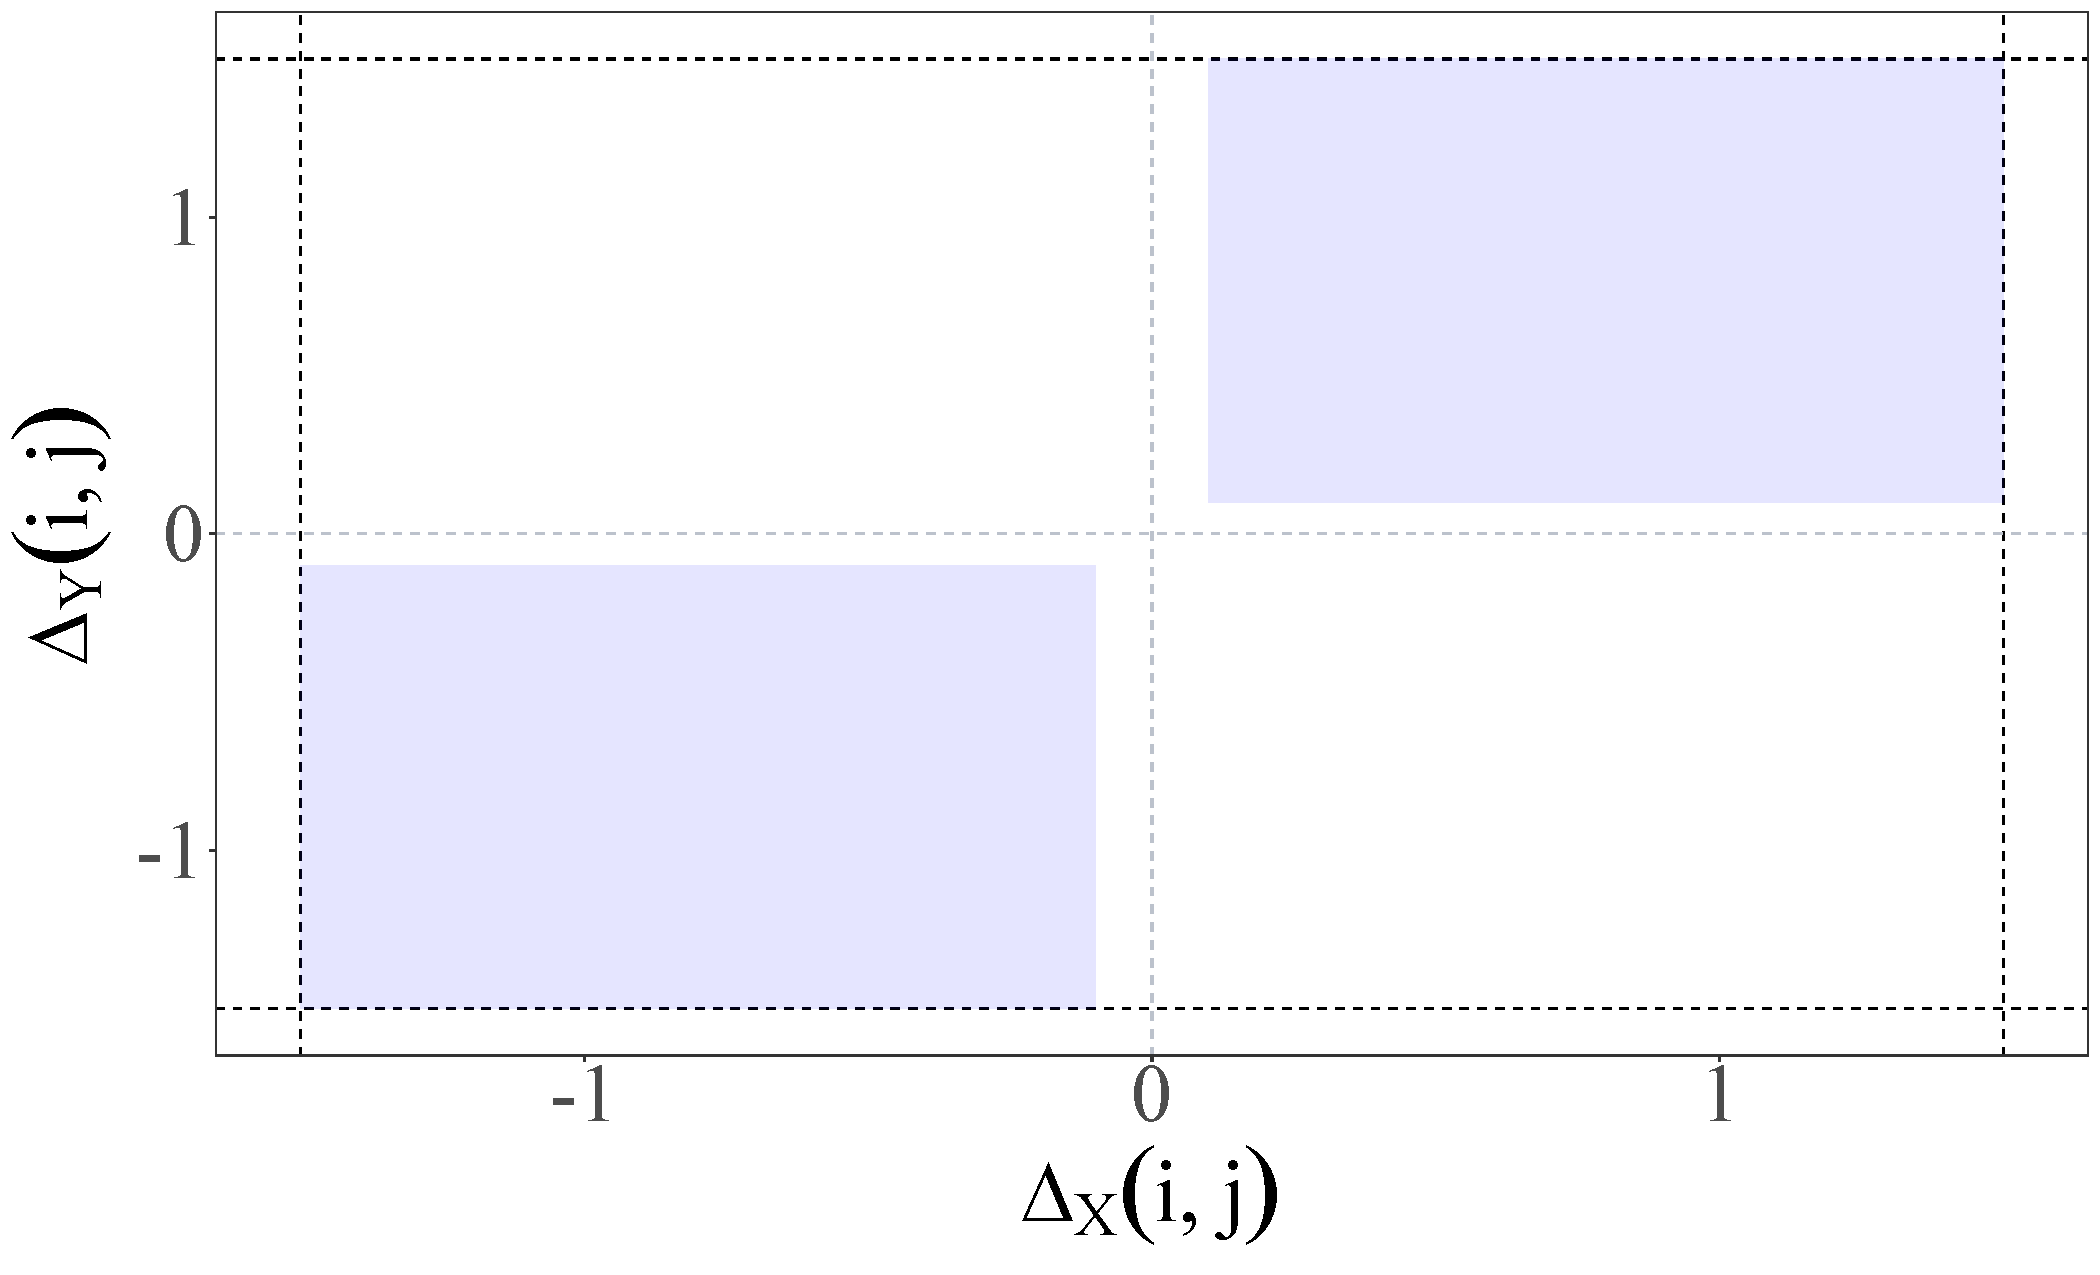
\includegraphics[width=\linewidth]{img/empty-butterfly}
				\onslide<3>
					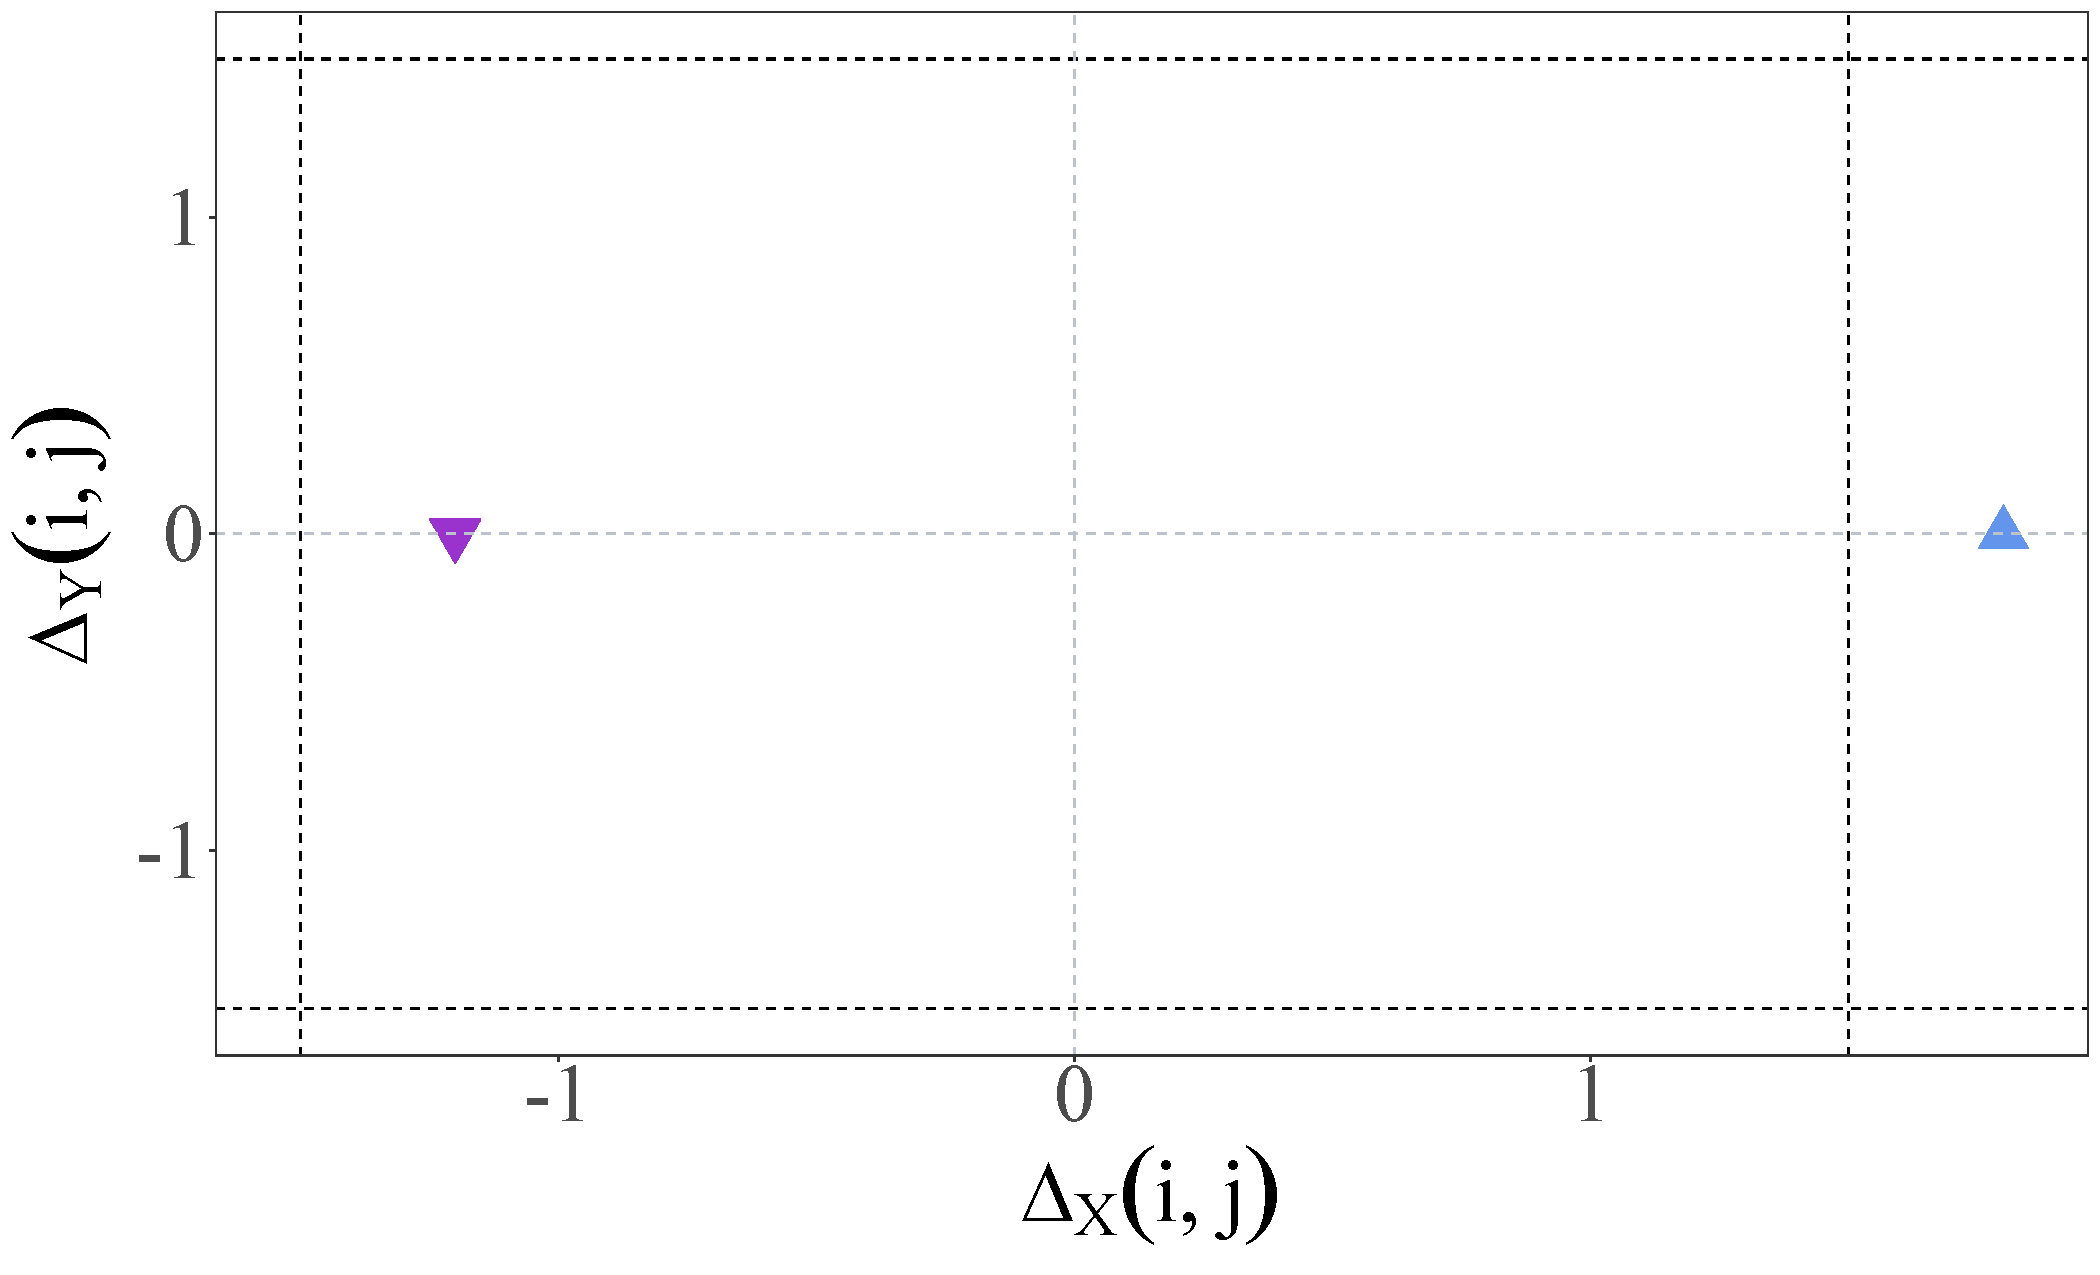
\includegraphics[width=\linewidth]{img/butterfly-01}
			\onslide<4>
					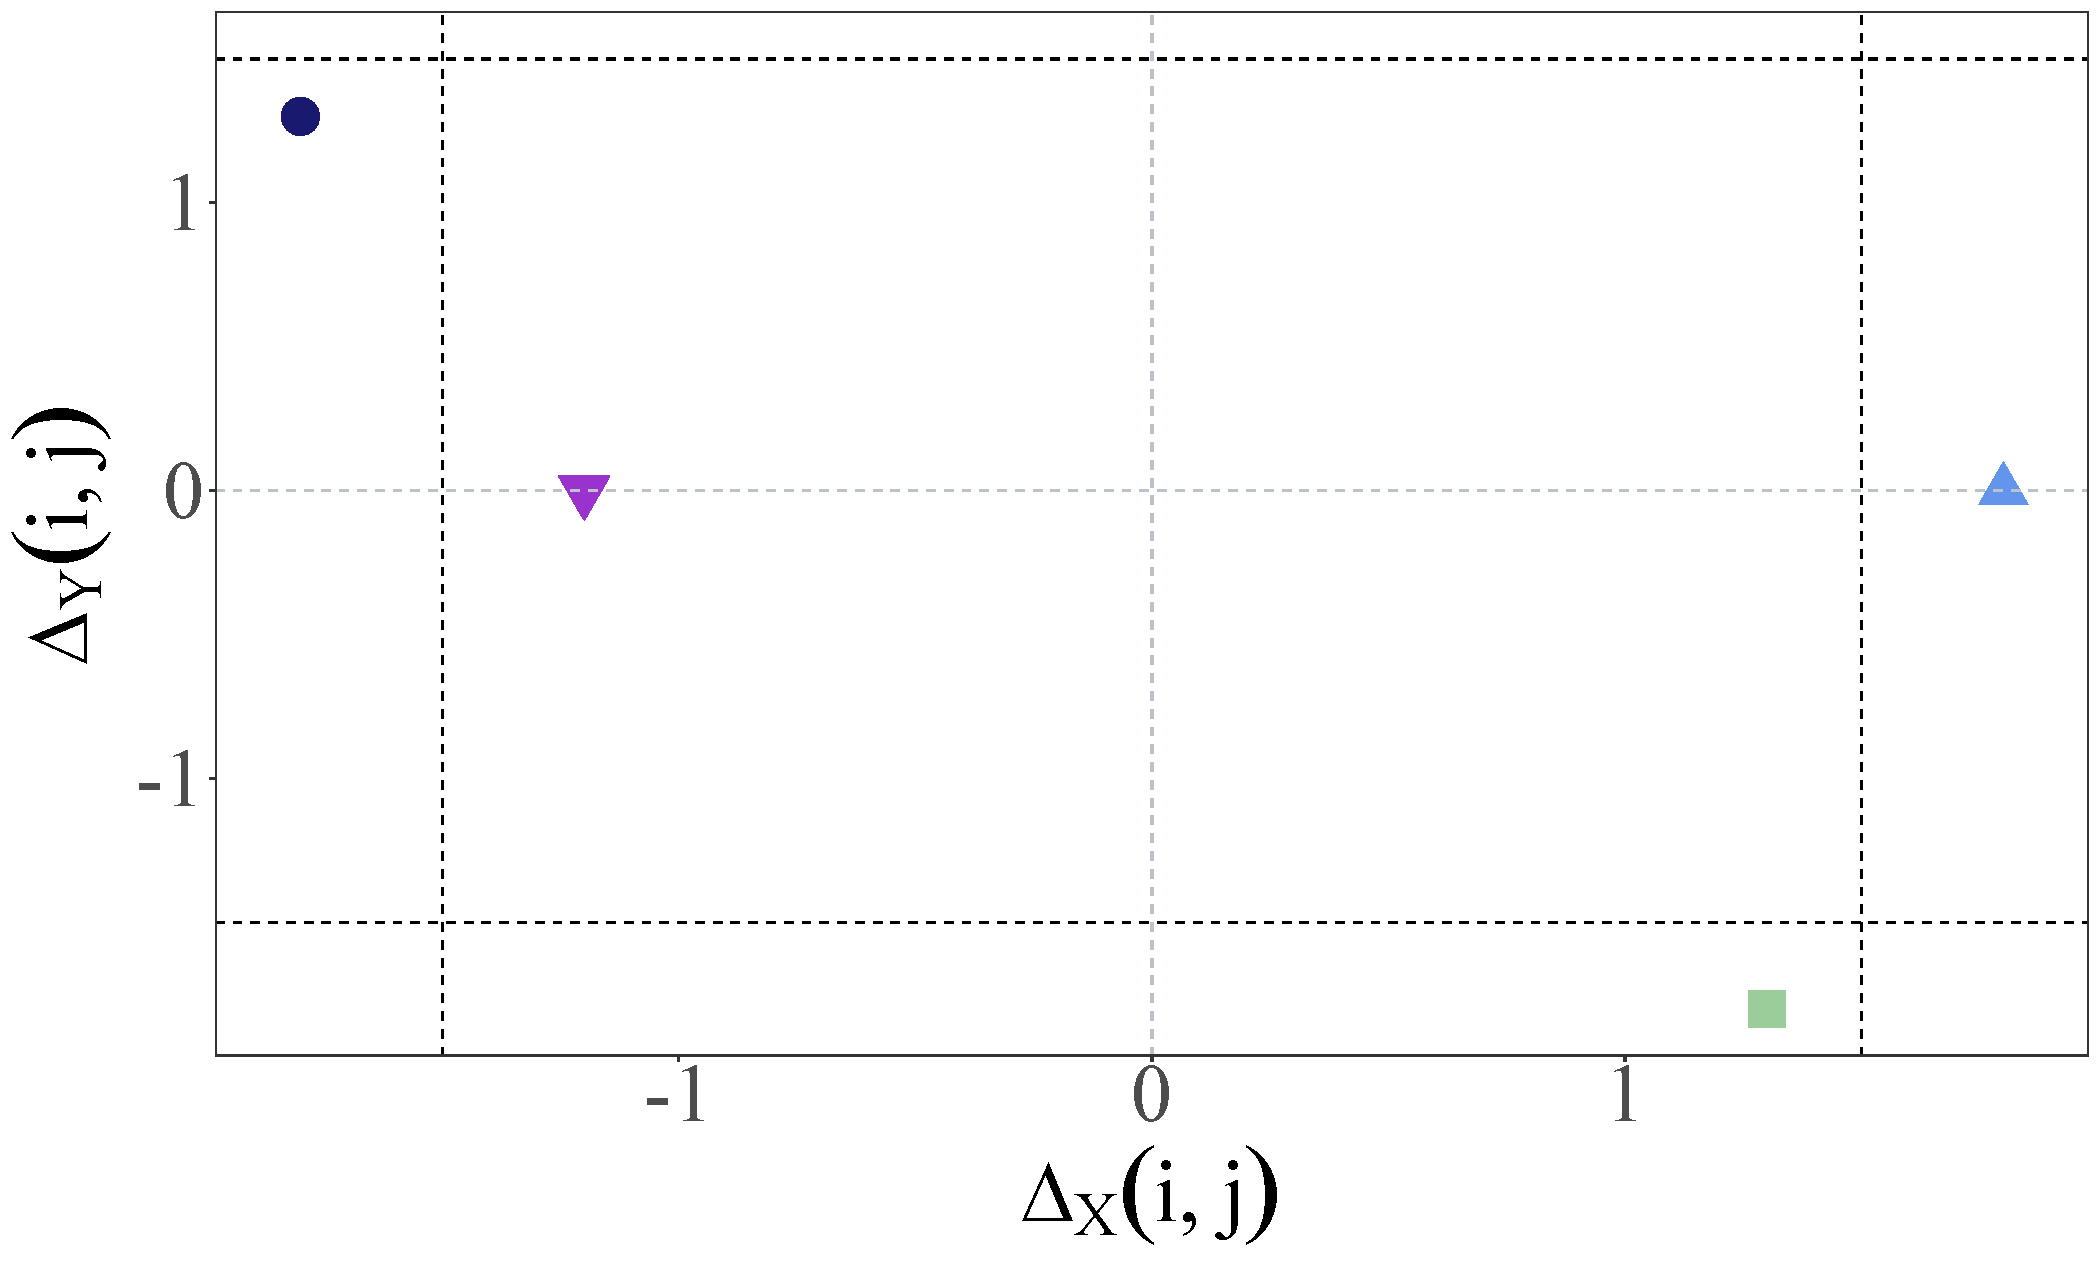
\includegraphics[width=\linewidth]{img/butterfly-02}
			\end{overprint}
		
		\end{column}
	\end{columns}

	
\end{frame}

\subsection{Group differences}


\begin{frame}
	
	
	\begin{center}
		\begin{itemize}
			\item[] $H_0$: $\mu_{g1} -\mu_{g2} = 0$
			\item[] $H_1$: $\mu_{g1} -\mu_{g2} \neq 0$
		\end{itemize}
		
	\end{center}

$t$-test on the standardized scores considering different grouping variables: 
\begin{table}
	\centering
	\begin{tabular}{l r r}
		\hline
		Grouping variable	&	$n_1$	&	$n_2$	\\\hline
		Gender	&	199	&	196	\\
		Administration order	&	202	&	193	\\
		Administration modality	&	211	&	184	\\
		Schooling years	&	171	&	224	\\
		\hline
	\end{tabular}
\end{table}


\end{frame}


\subsection{Results: Individual differences}



\begin{frame}{Attempt-based SM: Monotonic relation}
	
	\begin{columns}[T]
		\begin{column}{.50\linewidth}
			\centering
		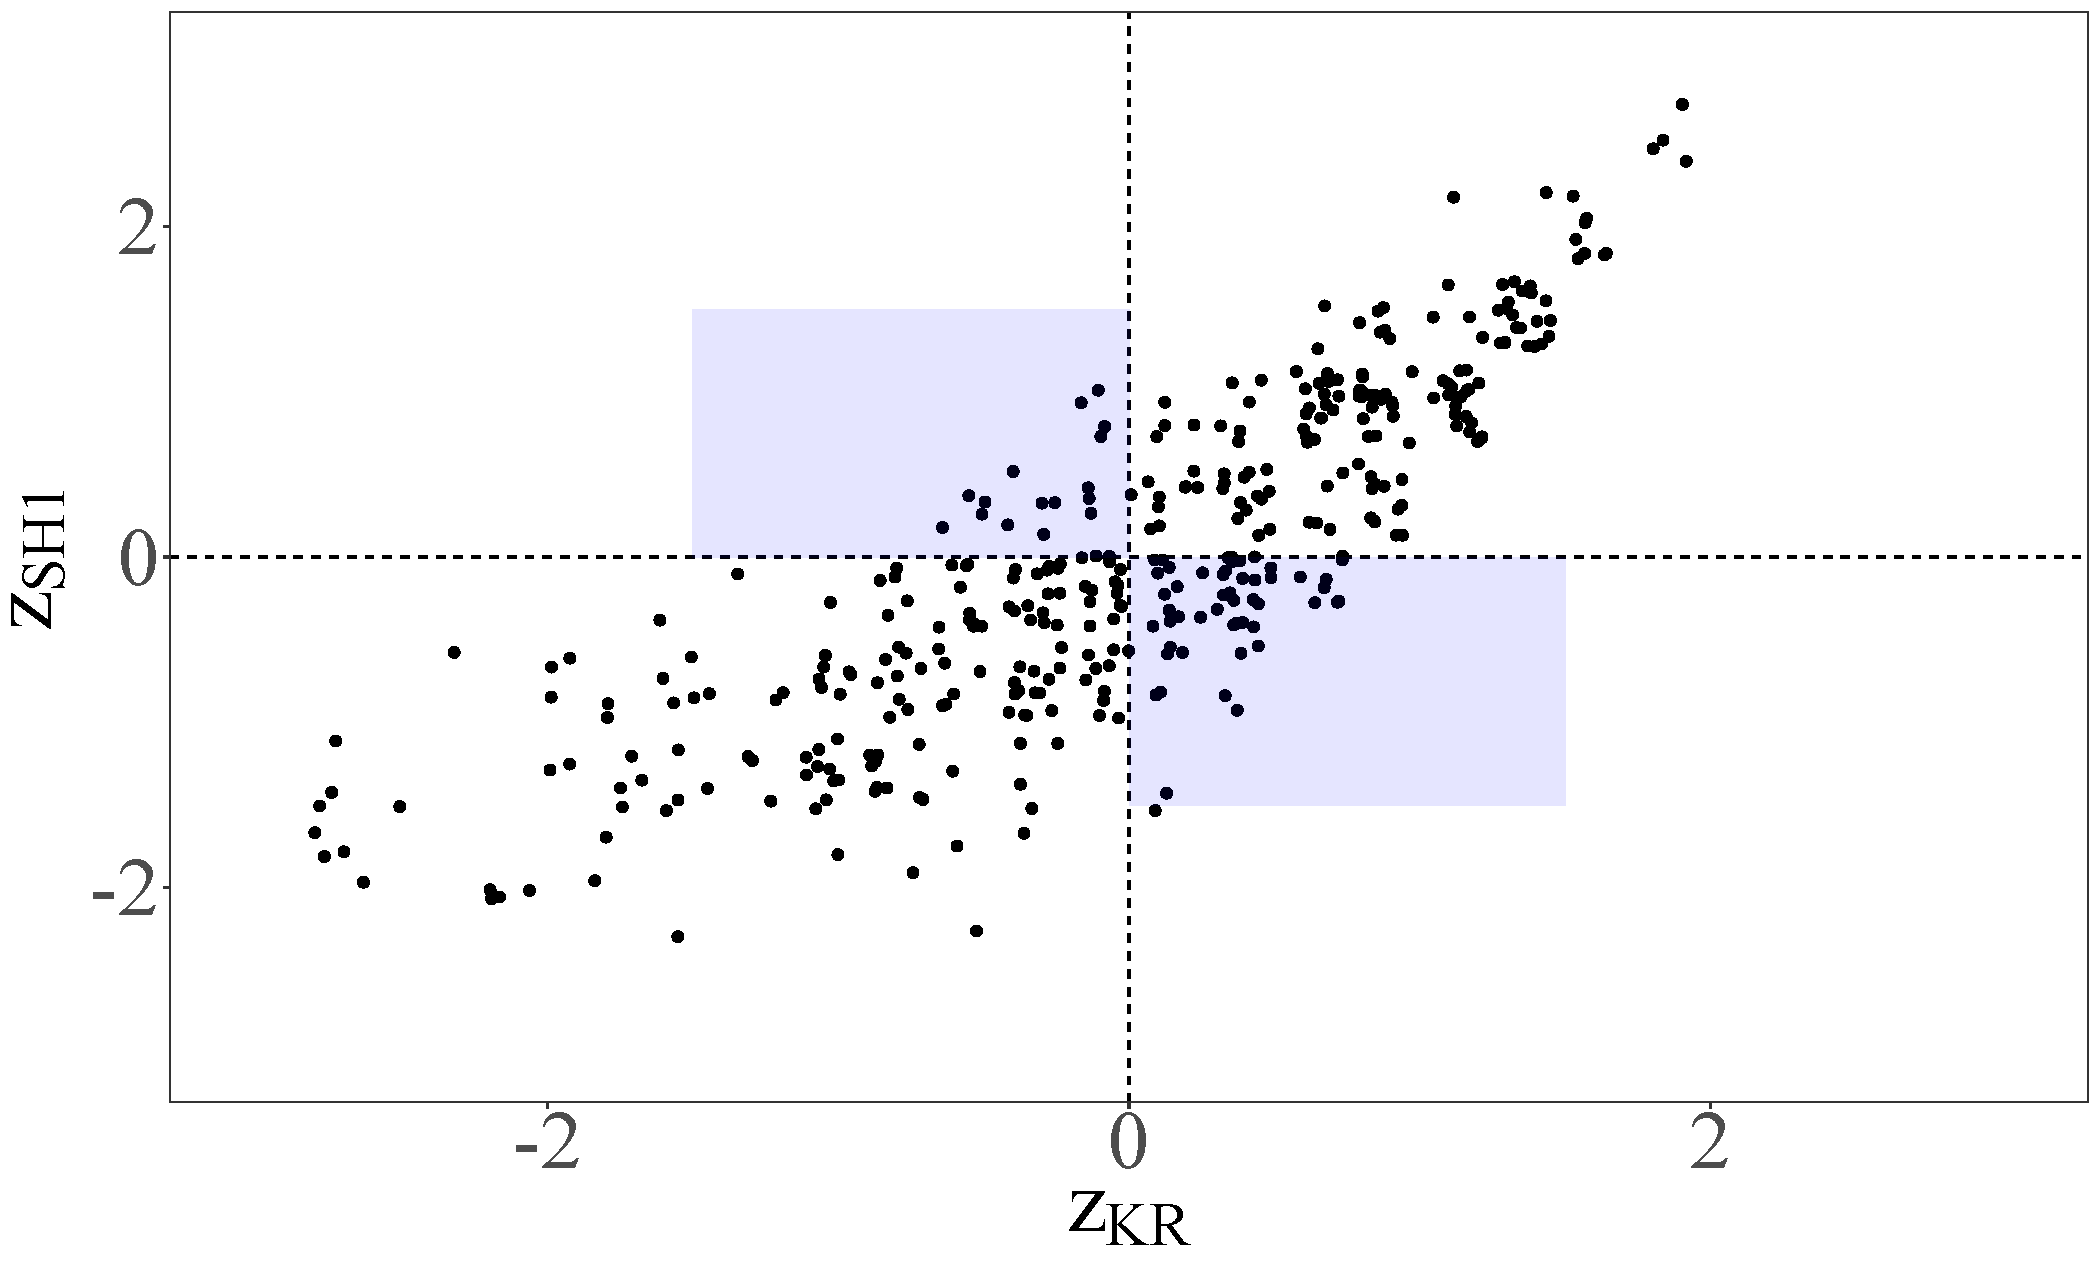
\includegraphics[width=\linewidth]{img/cor-KR-SH1}
		\end{column}
				\begin{column}{.50\linewidth}
					\centering
			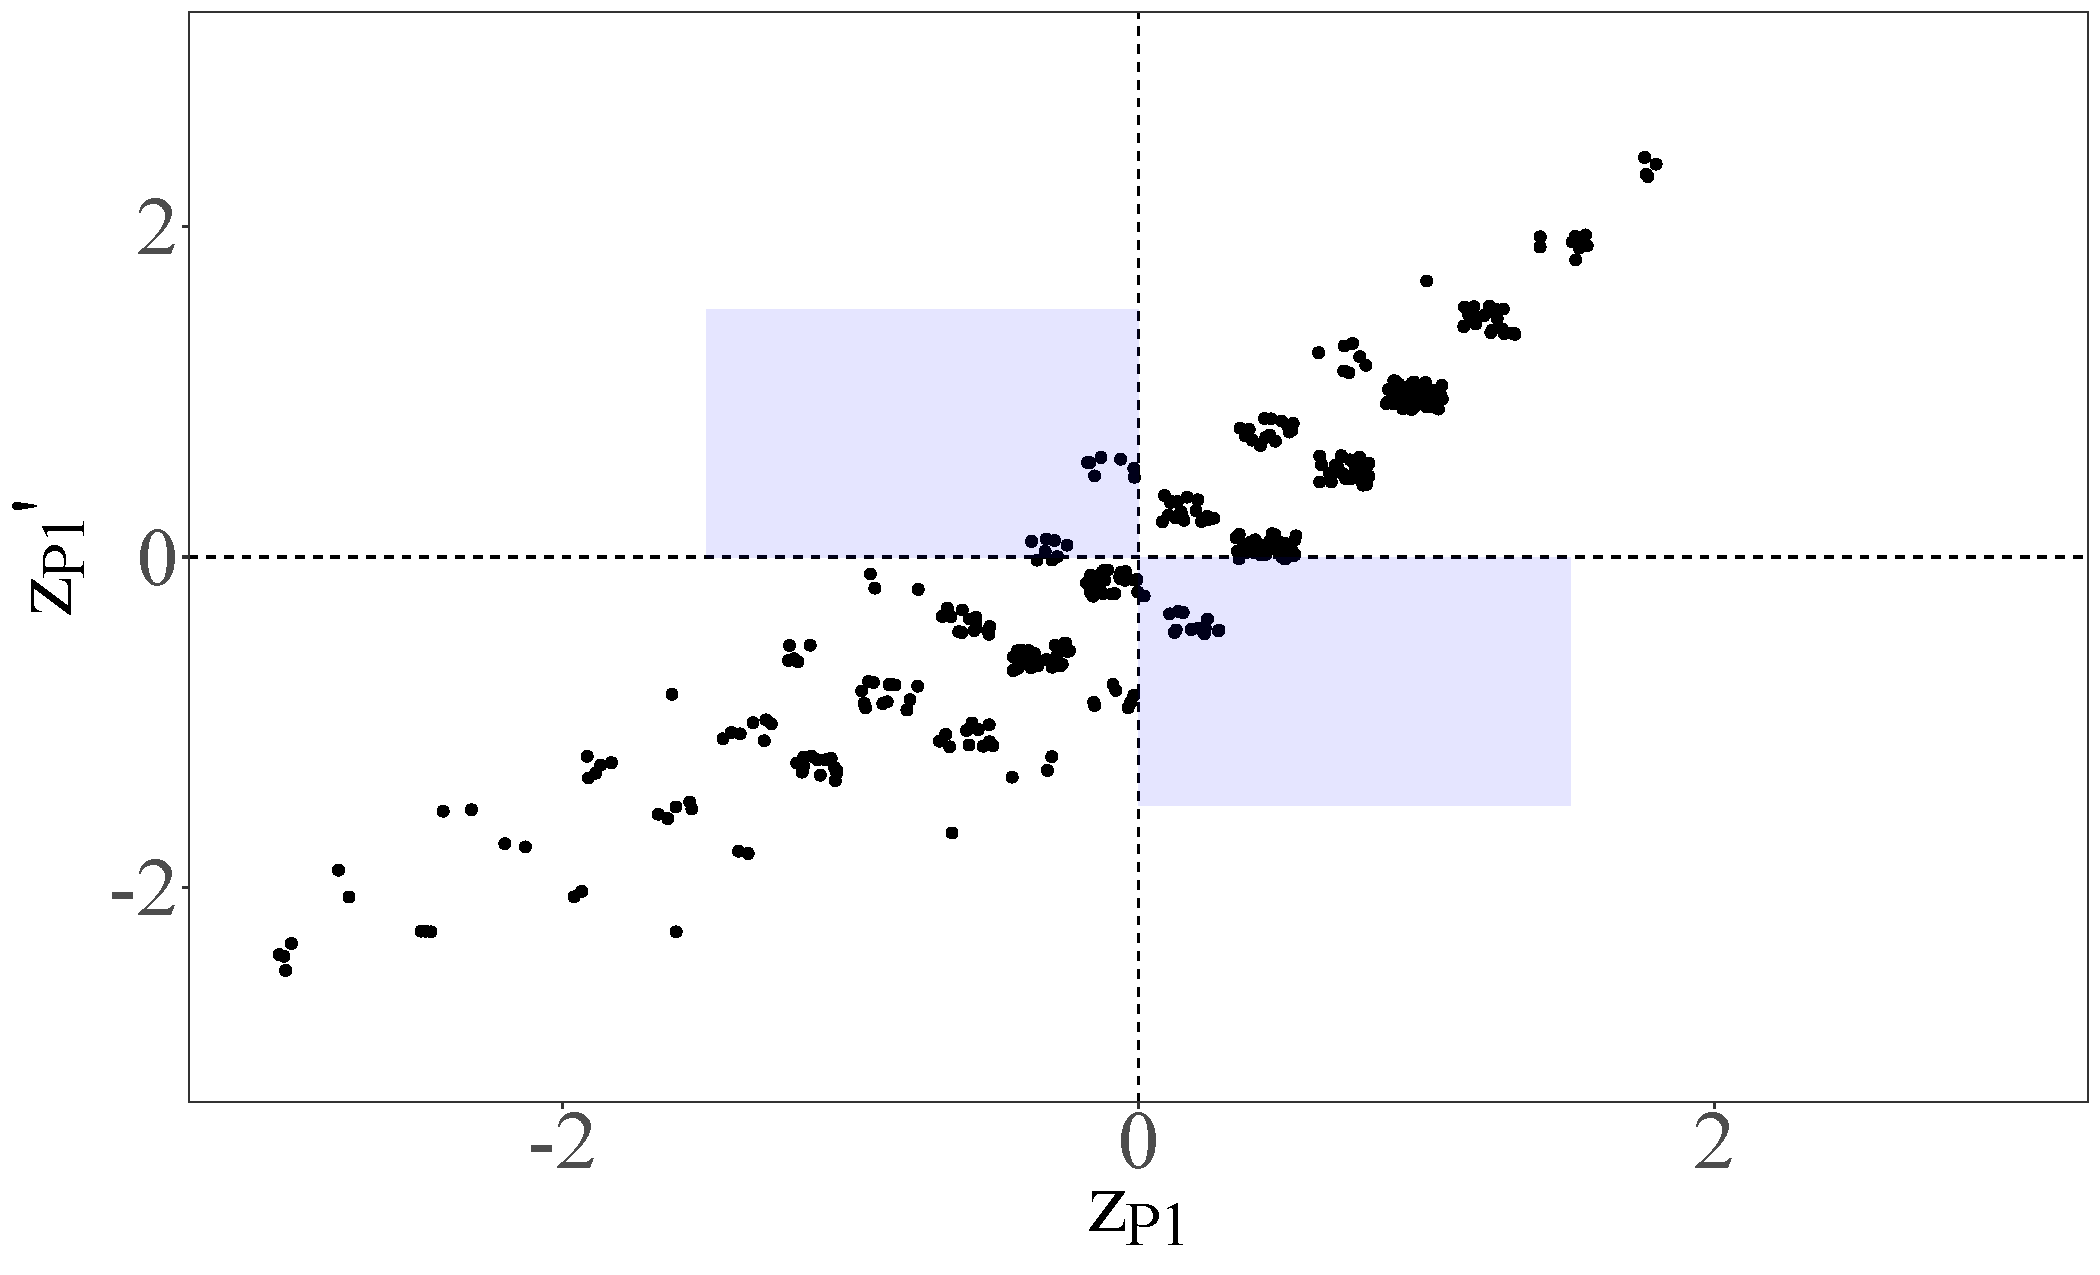
\includegraphics[width=\linewidth]{img/cor-P1-P1p}
		\end{column}
		
	\end{columns}
	


\end{frame}

 
 
 \begin{frame}{Attempt-based SM: Differences and distances}

 	\begin{columns}[T]
 		
 		\begin{column}{.50\linewidth}
 			\begin{overprint}
 				\onslide<1>
 				\centering
 				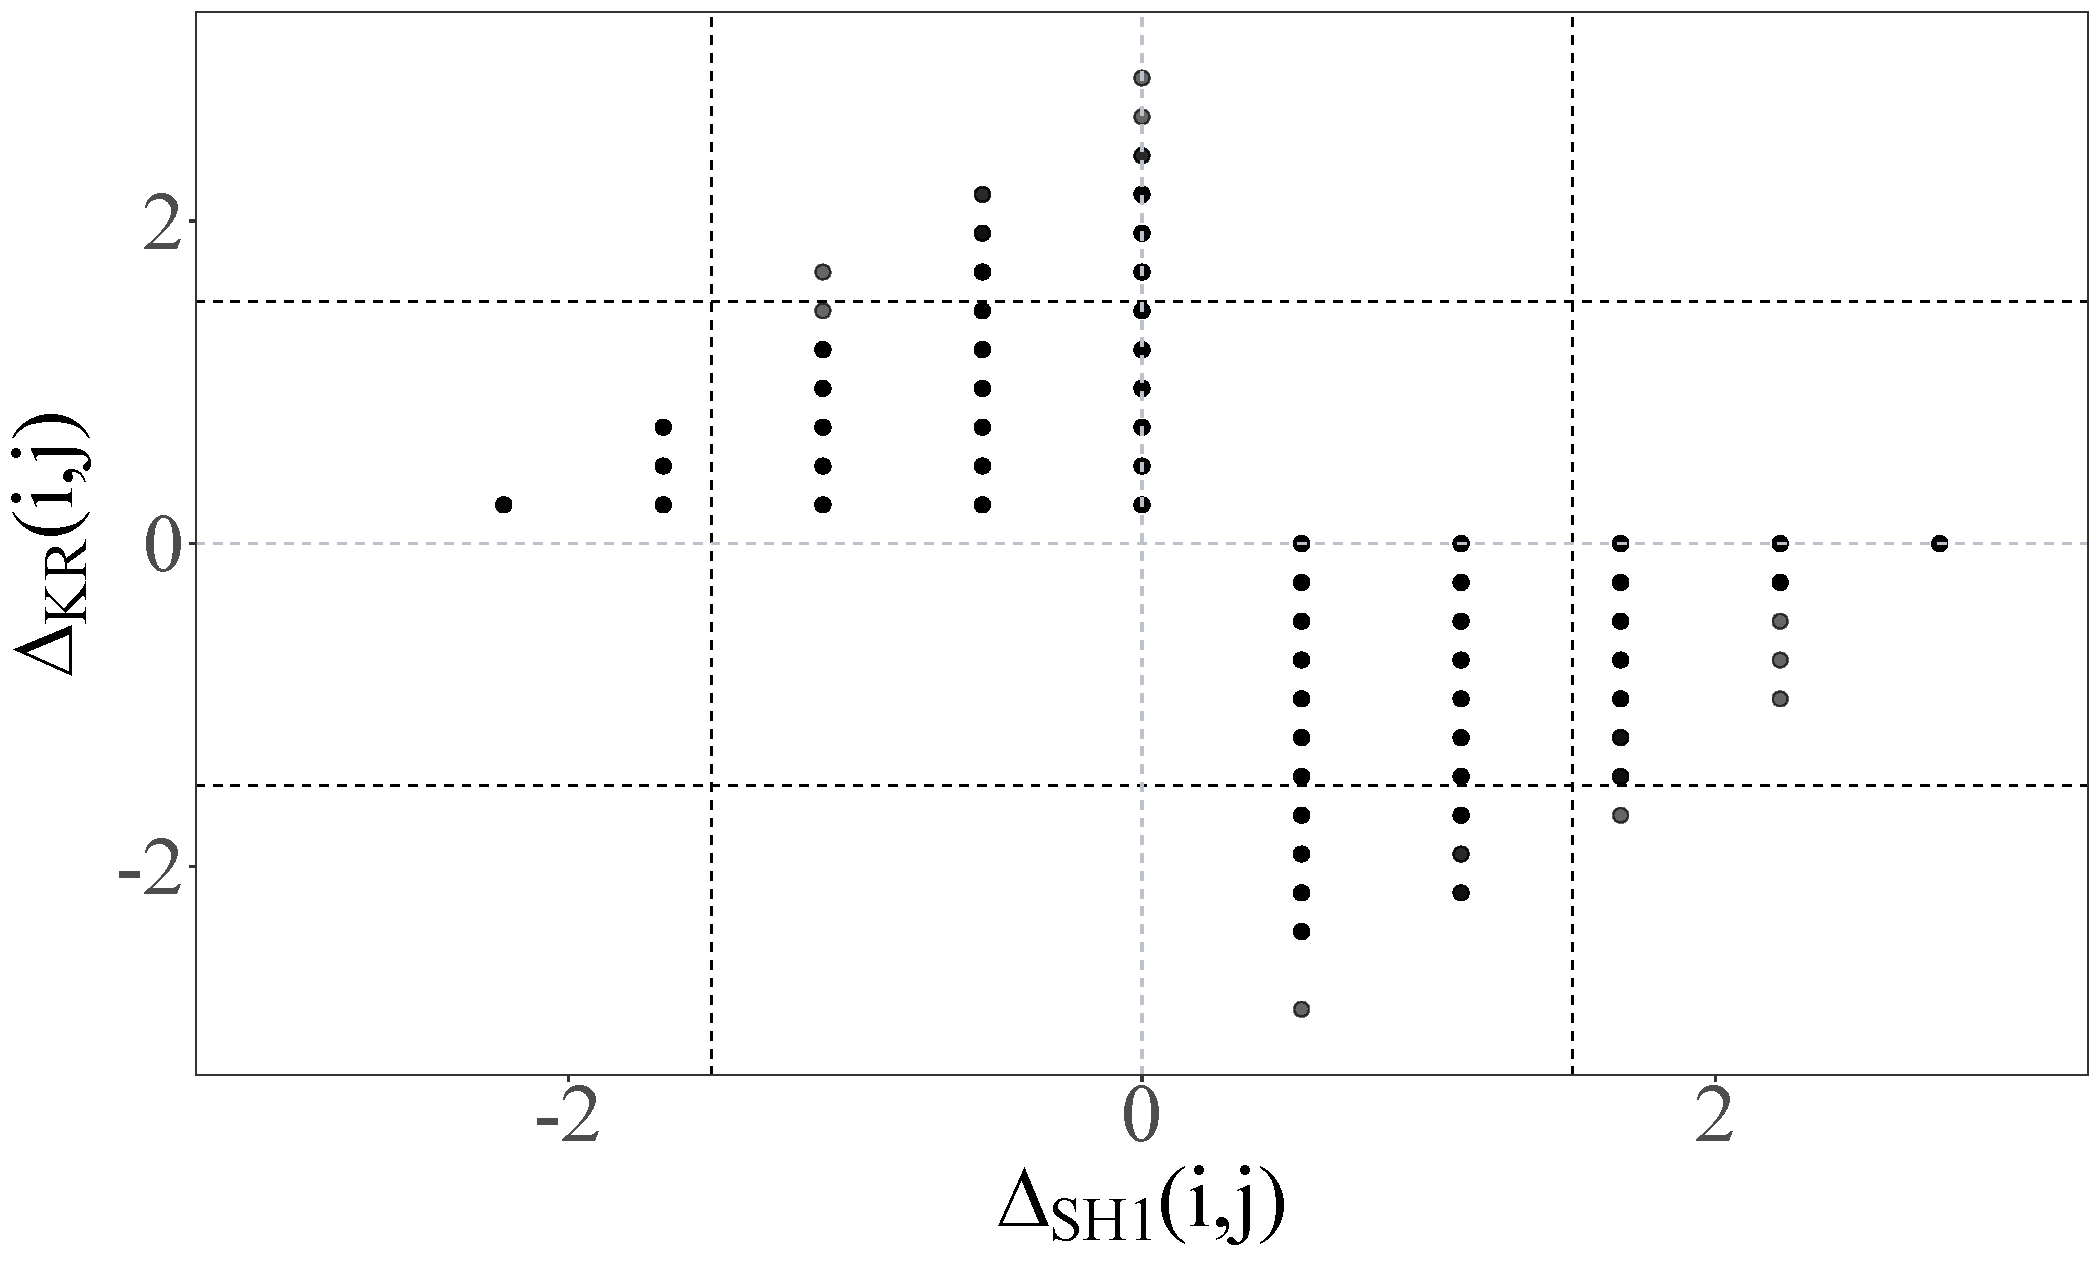
\includegraphics[width=\linewidth]{img/butterfly-SH1-KR}
 				\onslide<2>
 				\centering
 				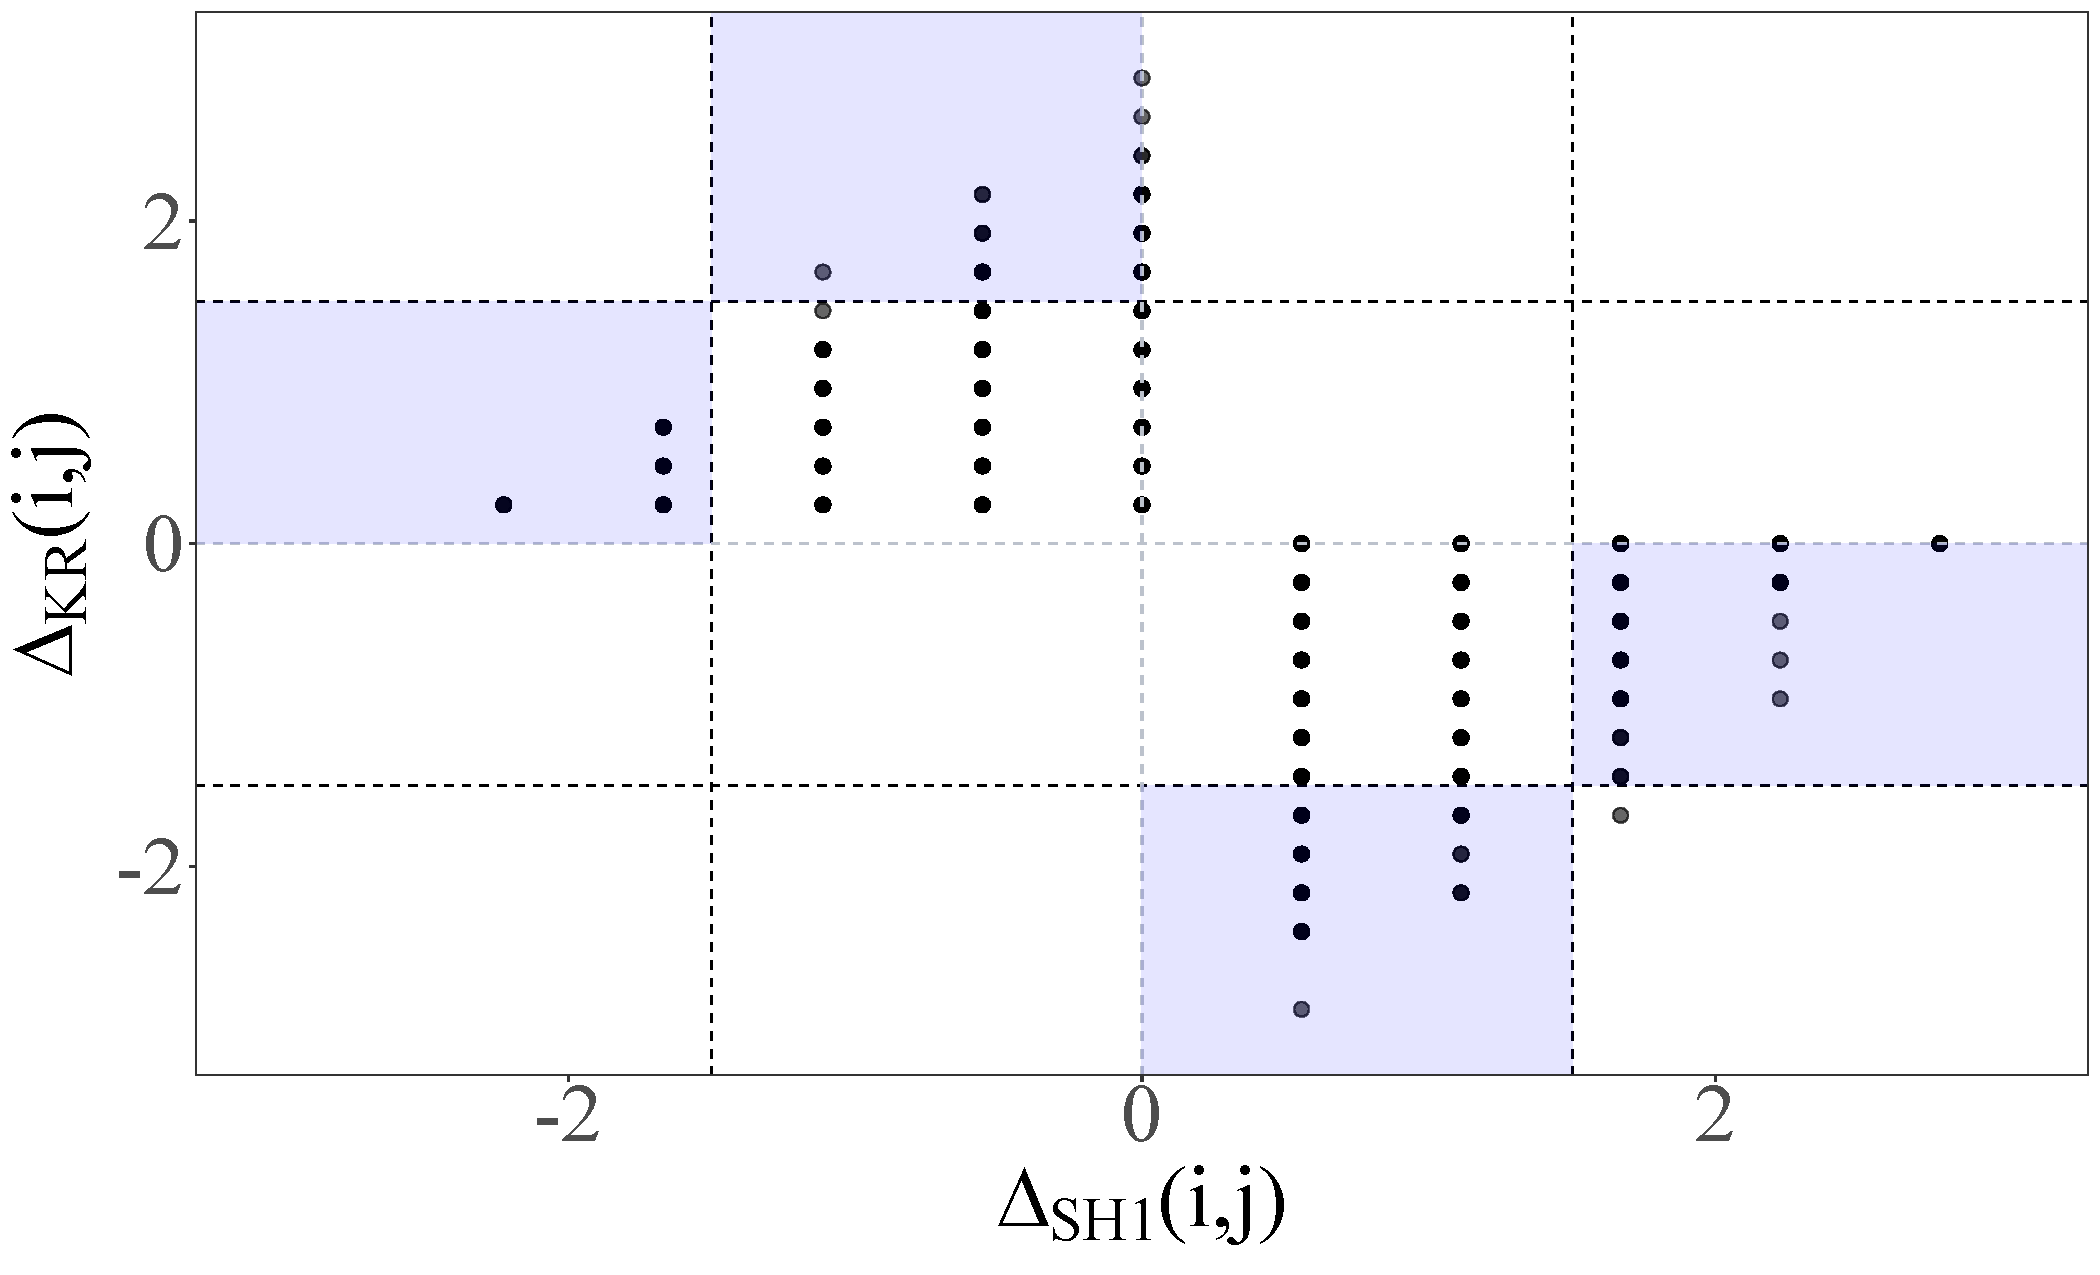
\includegraphics[width=\linewidth]{img/butterfly-SH1-KR-01}
 			\end{overprint}

 		\end{column}
 		\begin{column}{.50\linewidth}
 			 			\begin{overprint}
 				\onslide<1>
 				\centering
 				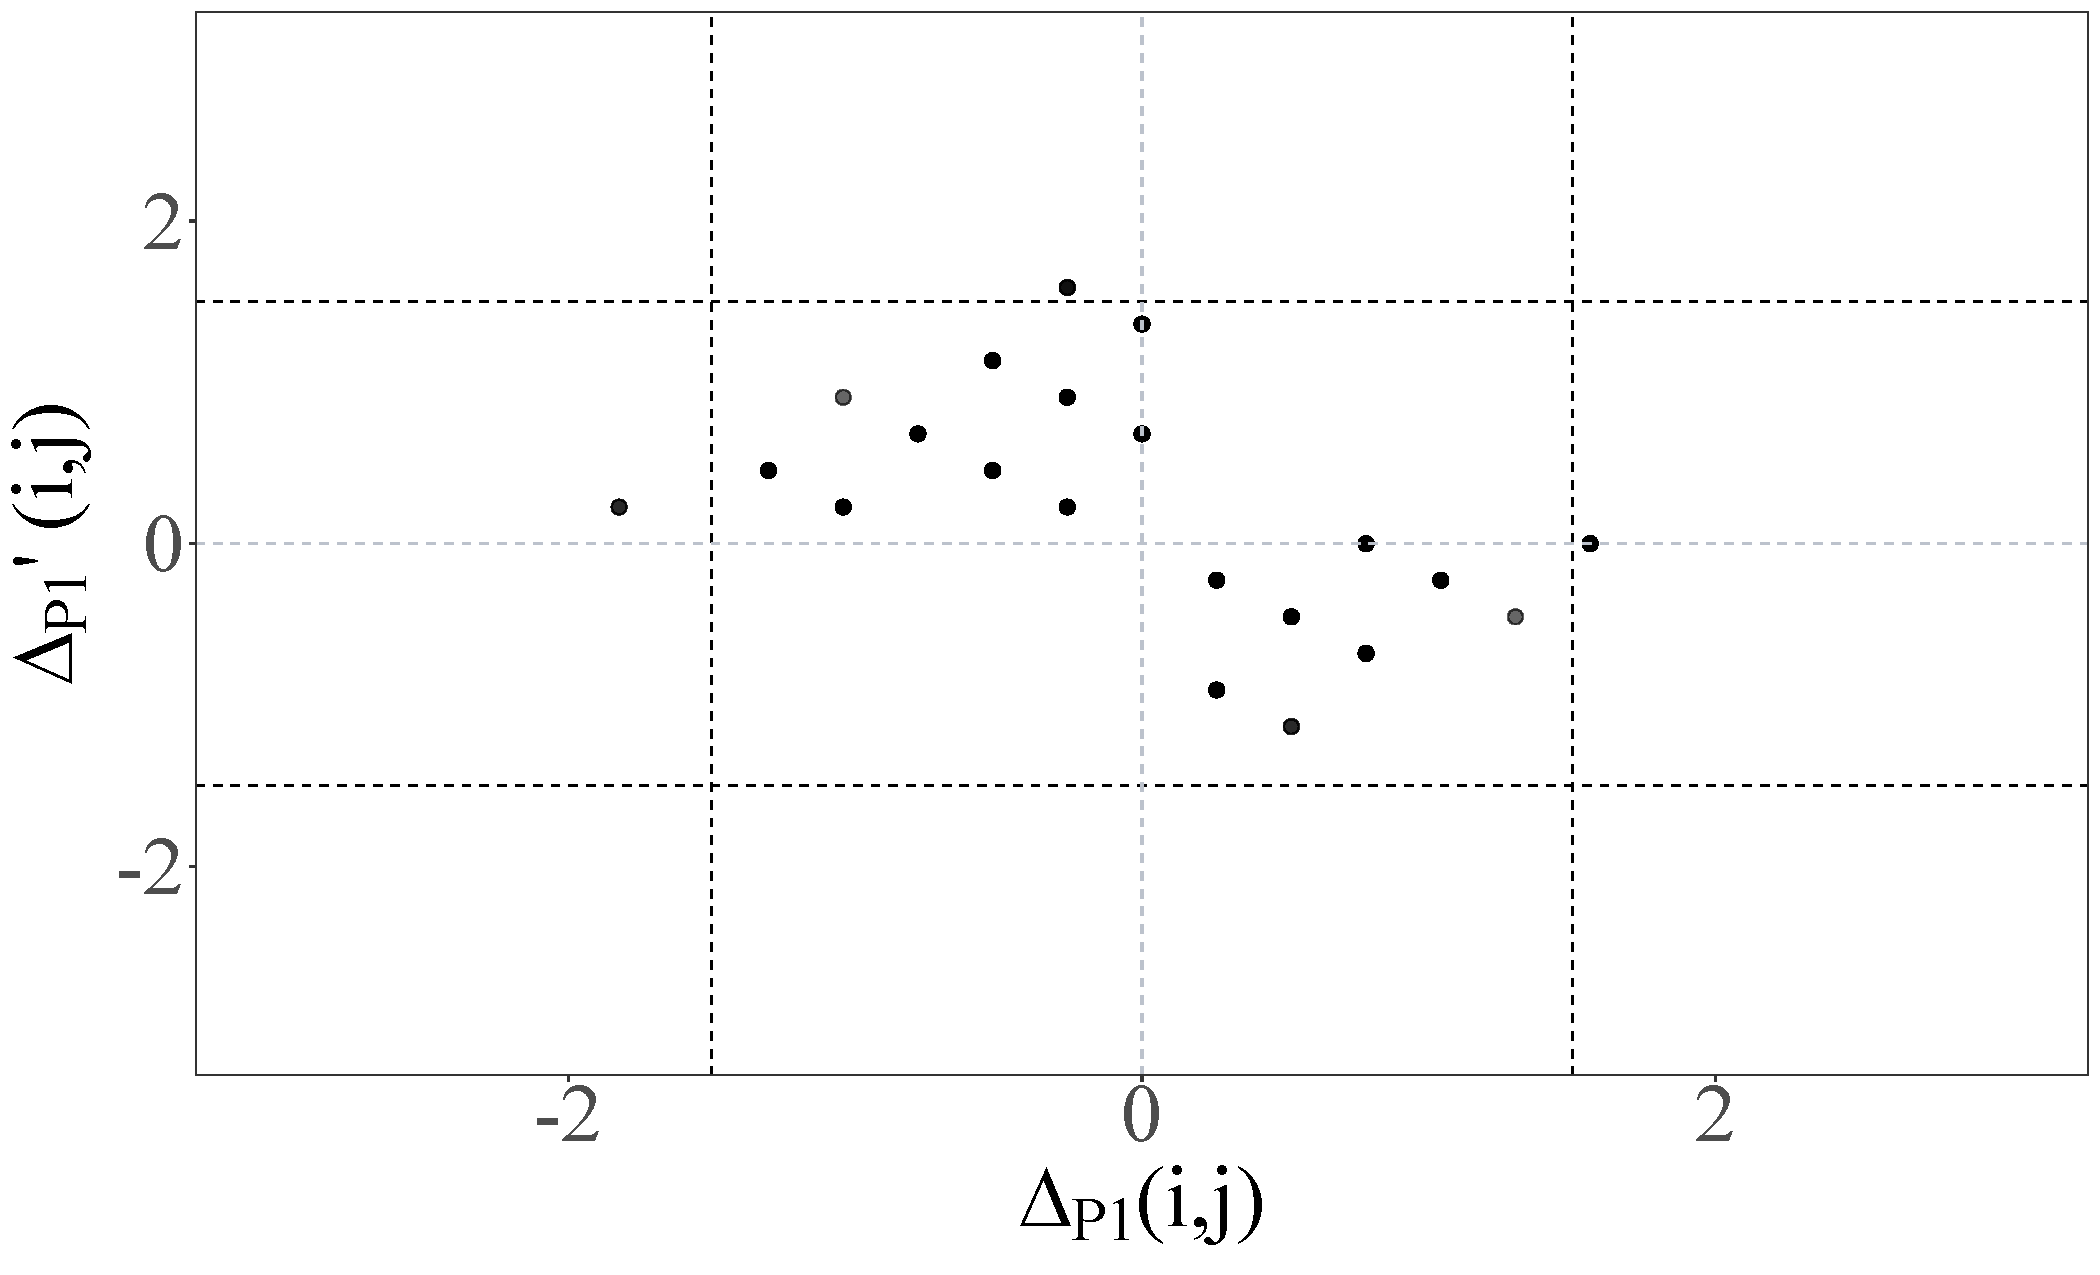
\includegraphics[width=\linewidth]{img/butterfly-P1-P1p}
 				\onslide<2>
 				\centering
 				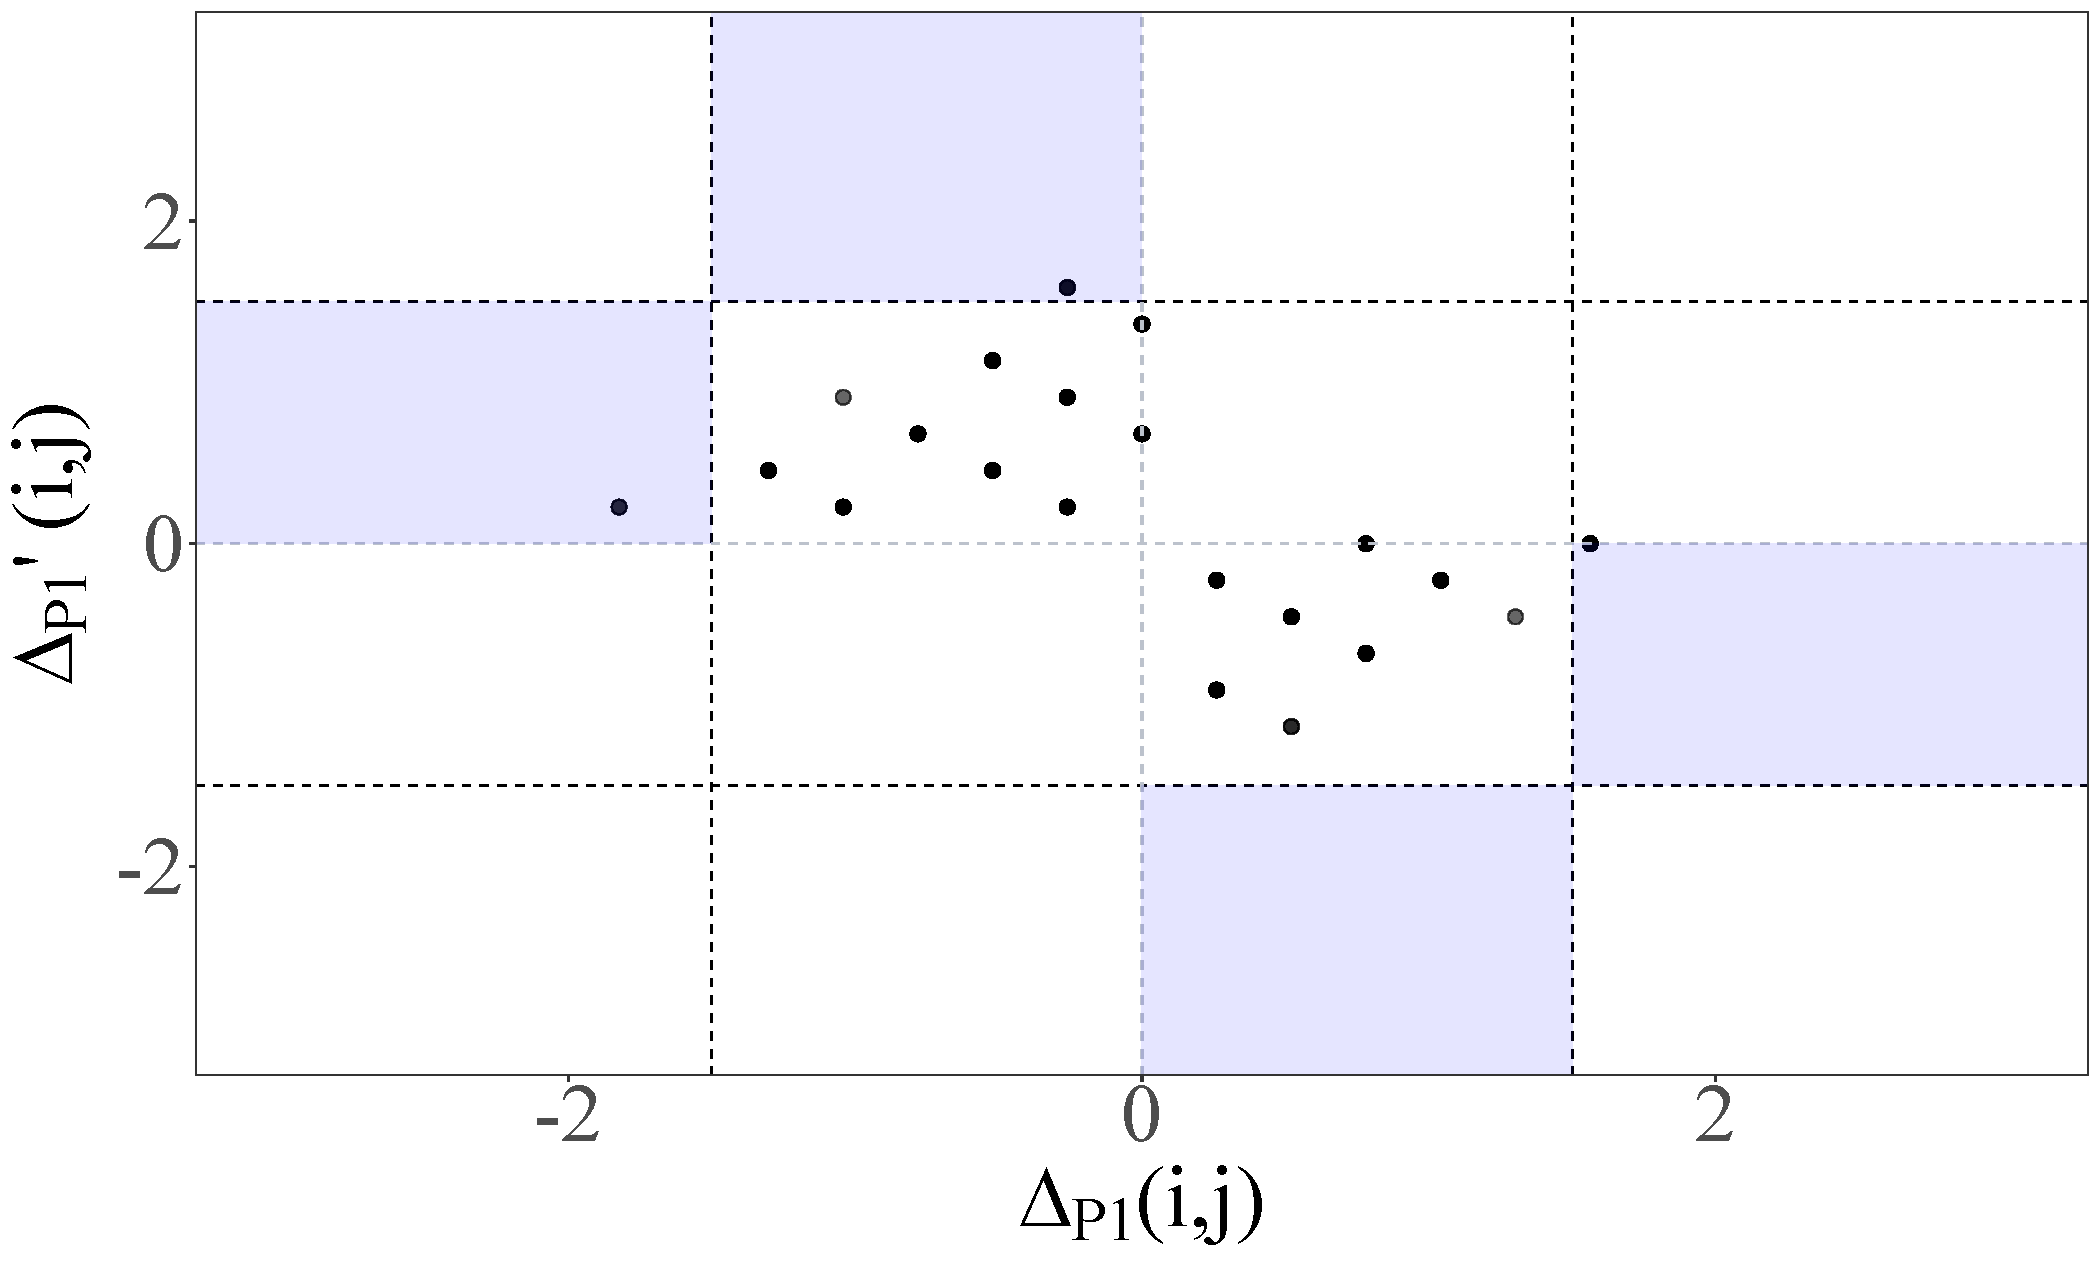
\includegraphics[width=\linewidth]{img/butterfly-P1-P1p-01}
 			\end{overprint}
 		\end{column}
 	\end{columns}
 	
 	
 \end{frame}
 
 \begin{frame}{Latency-based SM: Monotonic relation}
 	
 	\begin{columns}[T]
 		\begin{column}{.50\linewidth}
 			\centering
 			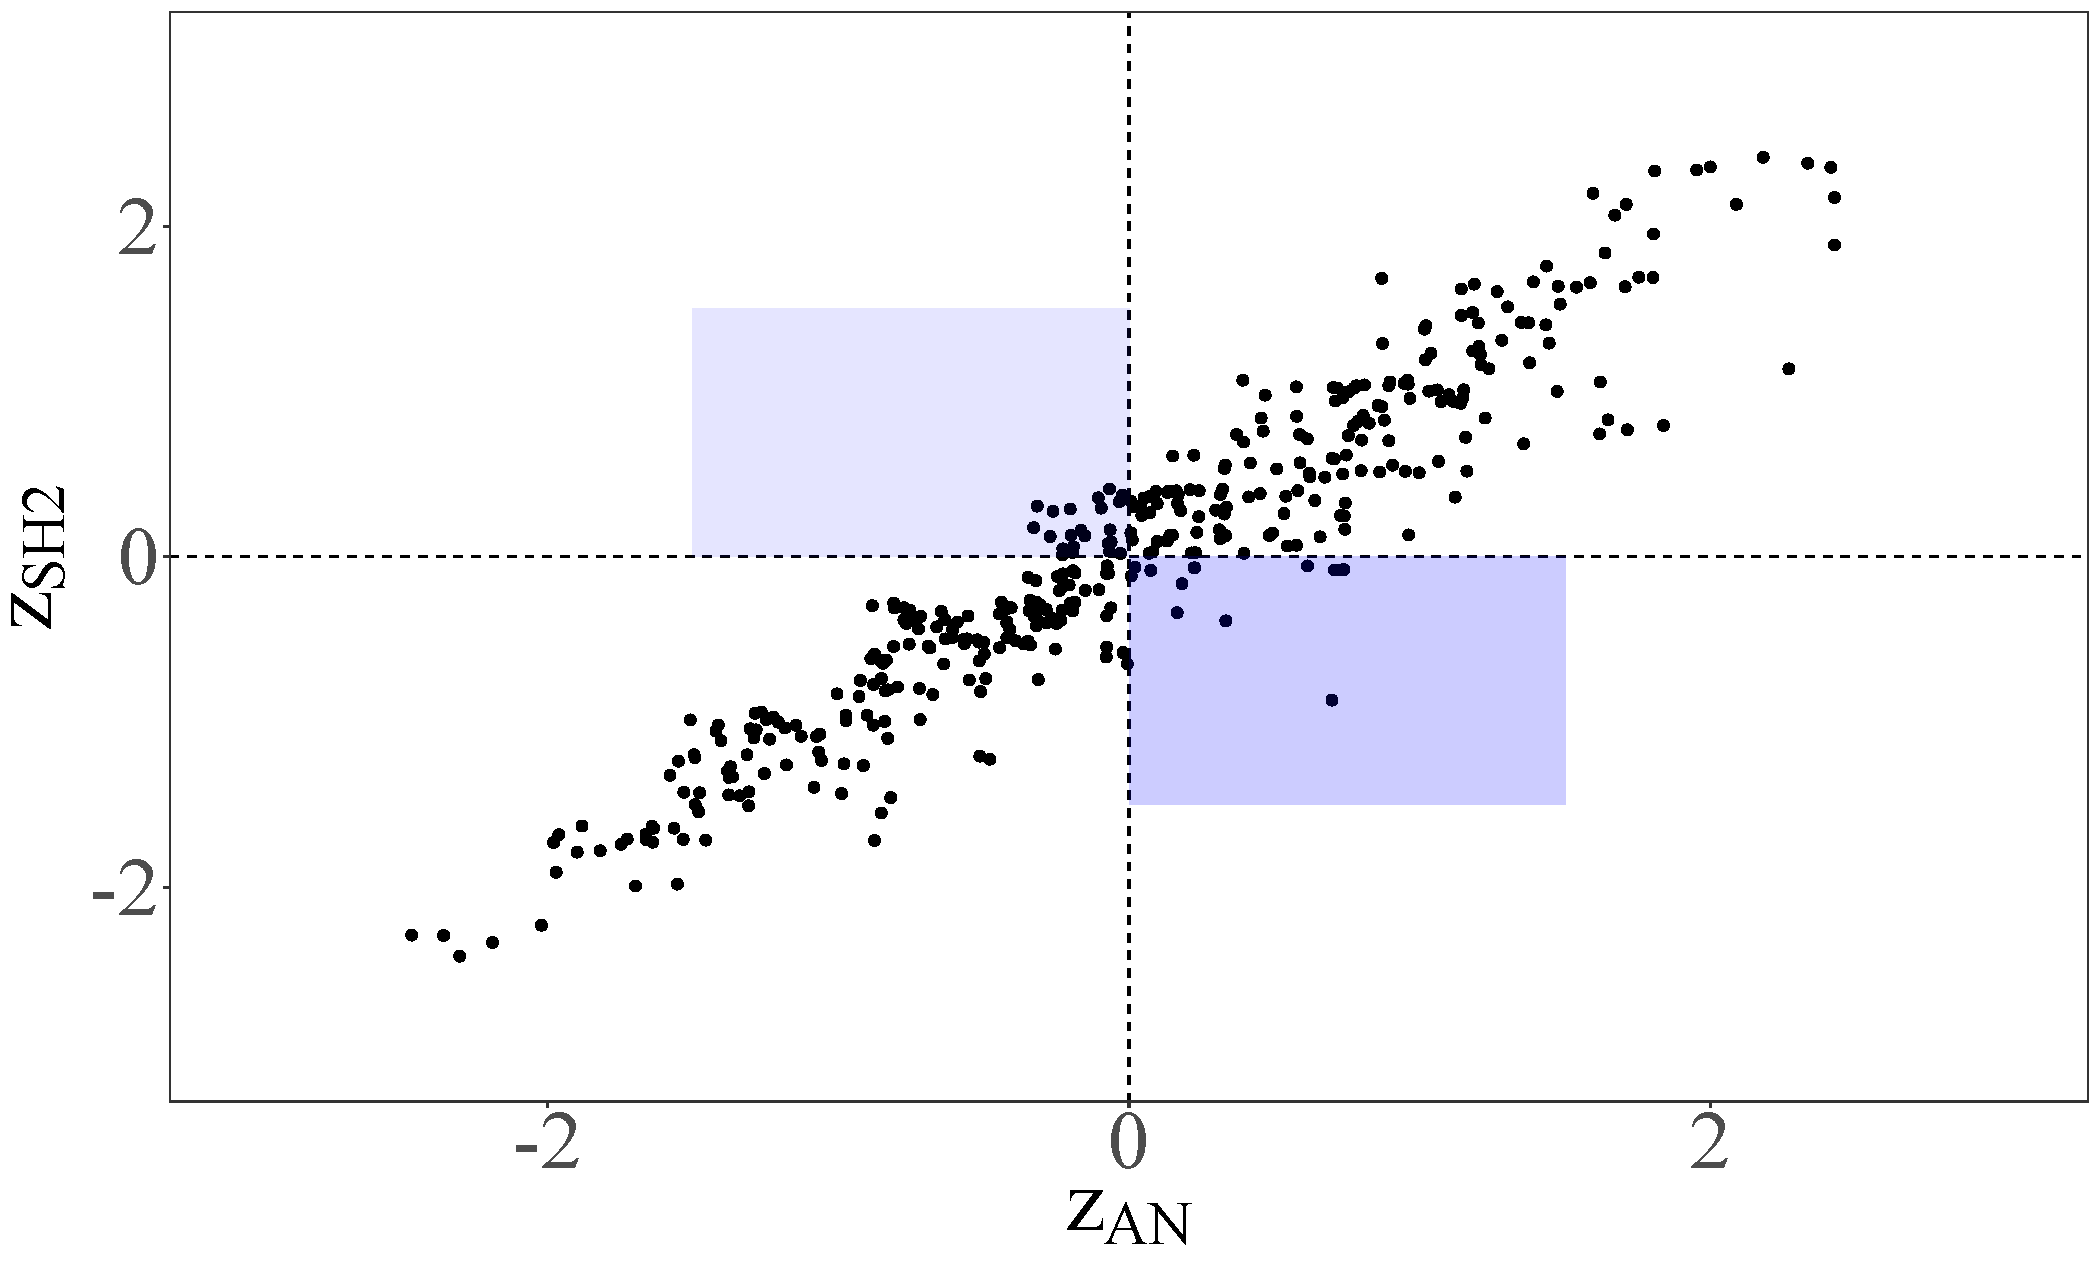
\includegraphics[width=\linewidth]{img/cor-AN-SH2}
 		\end{column}
 		\begin{column}{.50\linewidth}
 			\centering
 			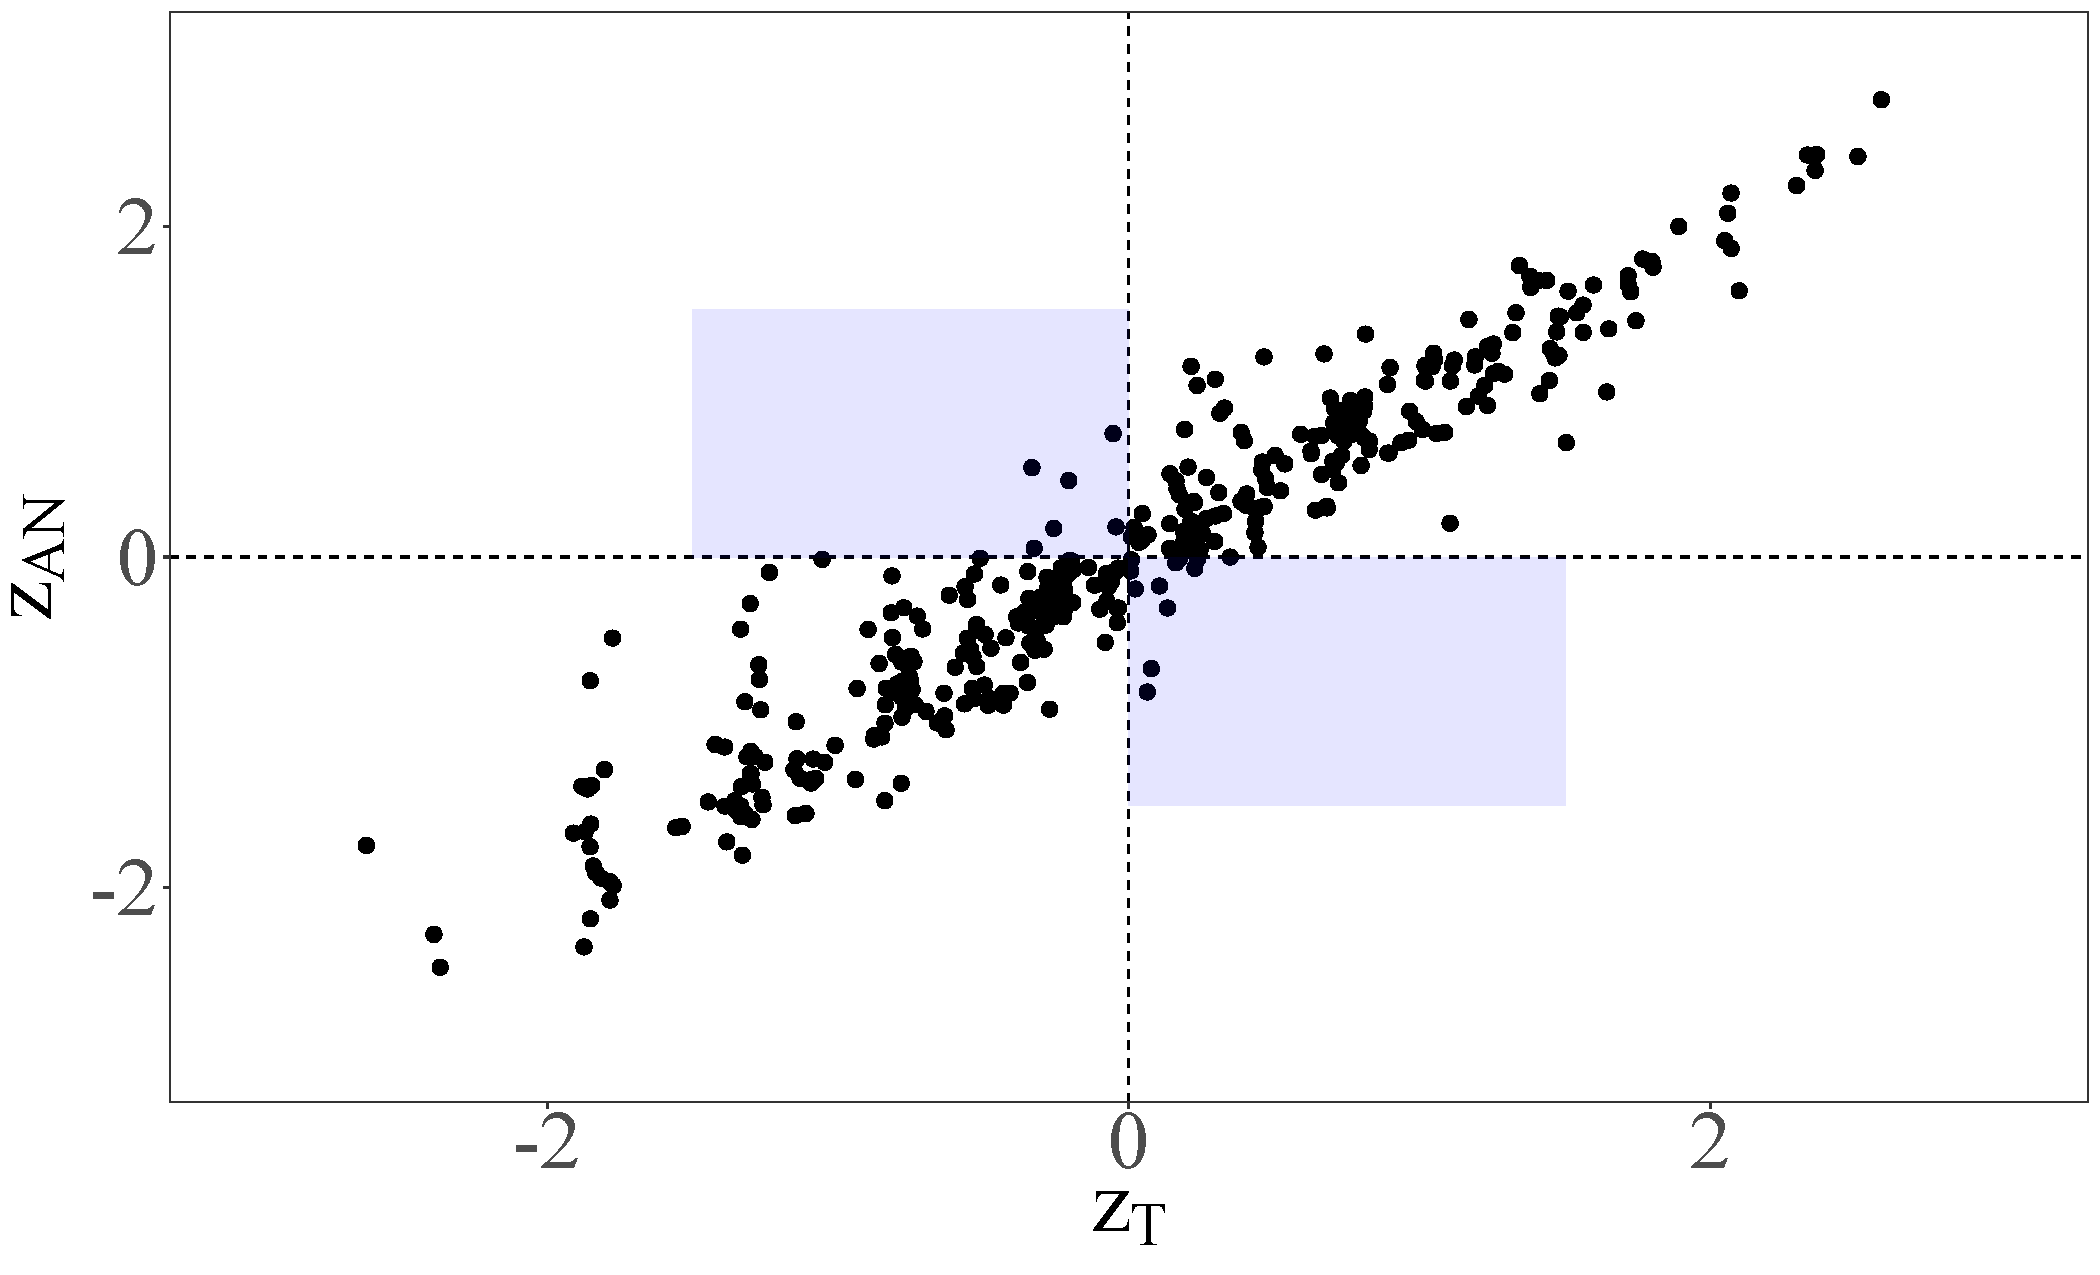
\includegraphics[width=\linewidth]{img/cor-T-AN}
 		\end{column}
 		
 	\end{columns}
 	
 	
 	
 \end{frame}
 
 
 
 \begin{frame}{Latency-based SM: Differences and distances}
 	
 	\begin{columns}[T]
 		
 		\begin{column}{.50\linewidth}
 			\begin{overprint}
 				\onslide<1>
 				\centering
 				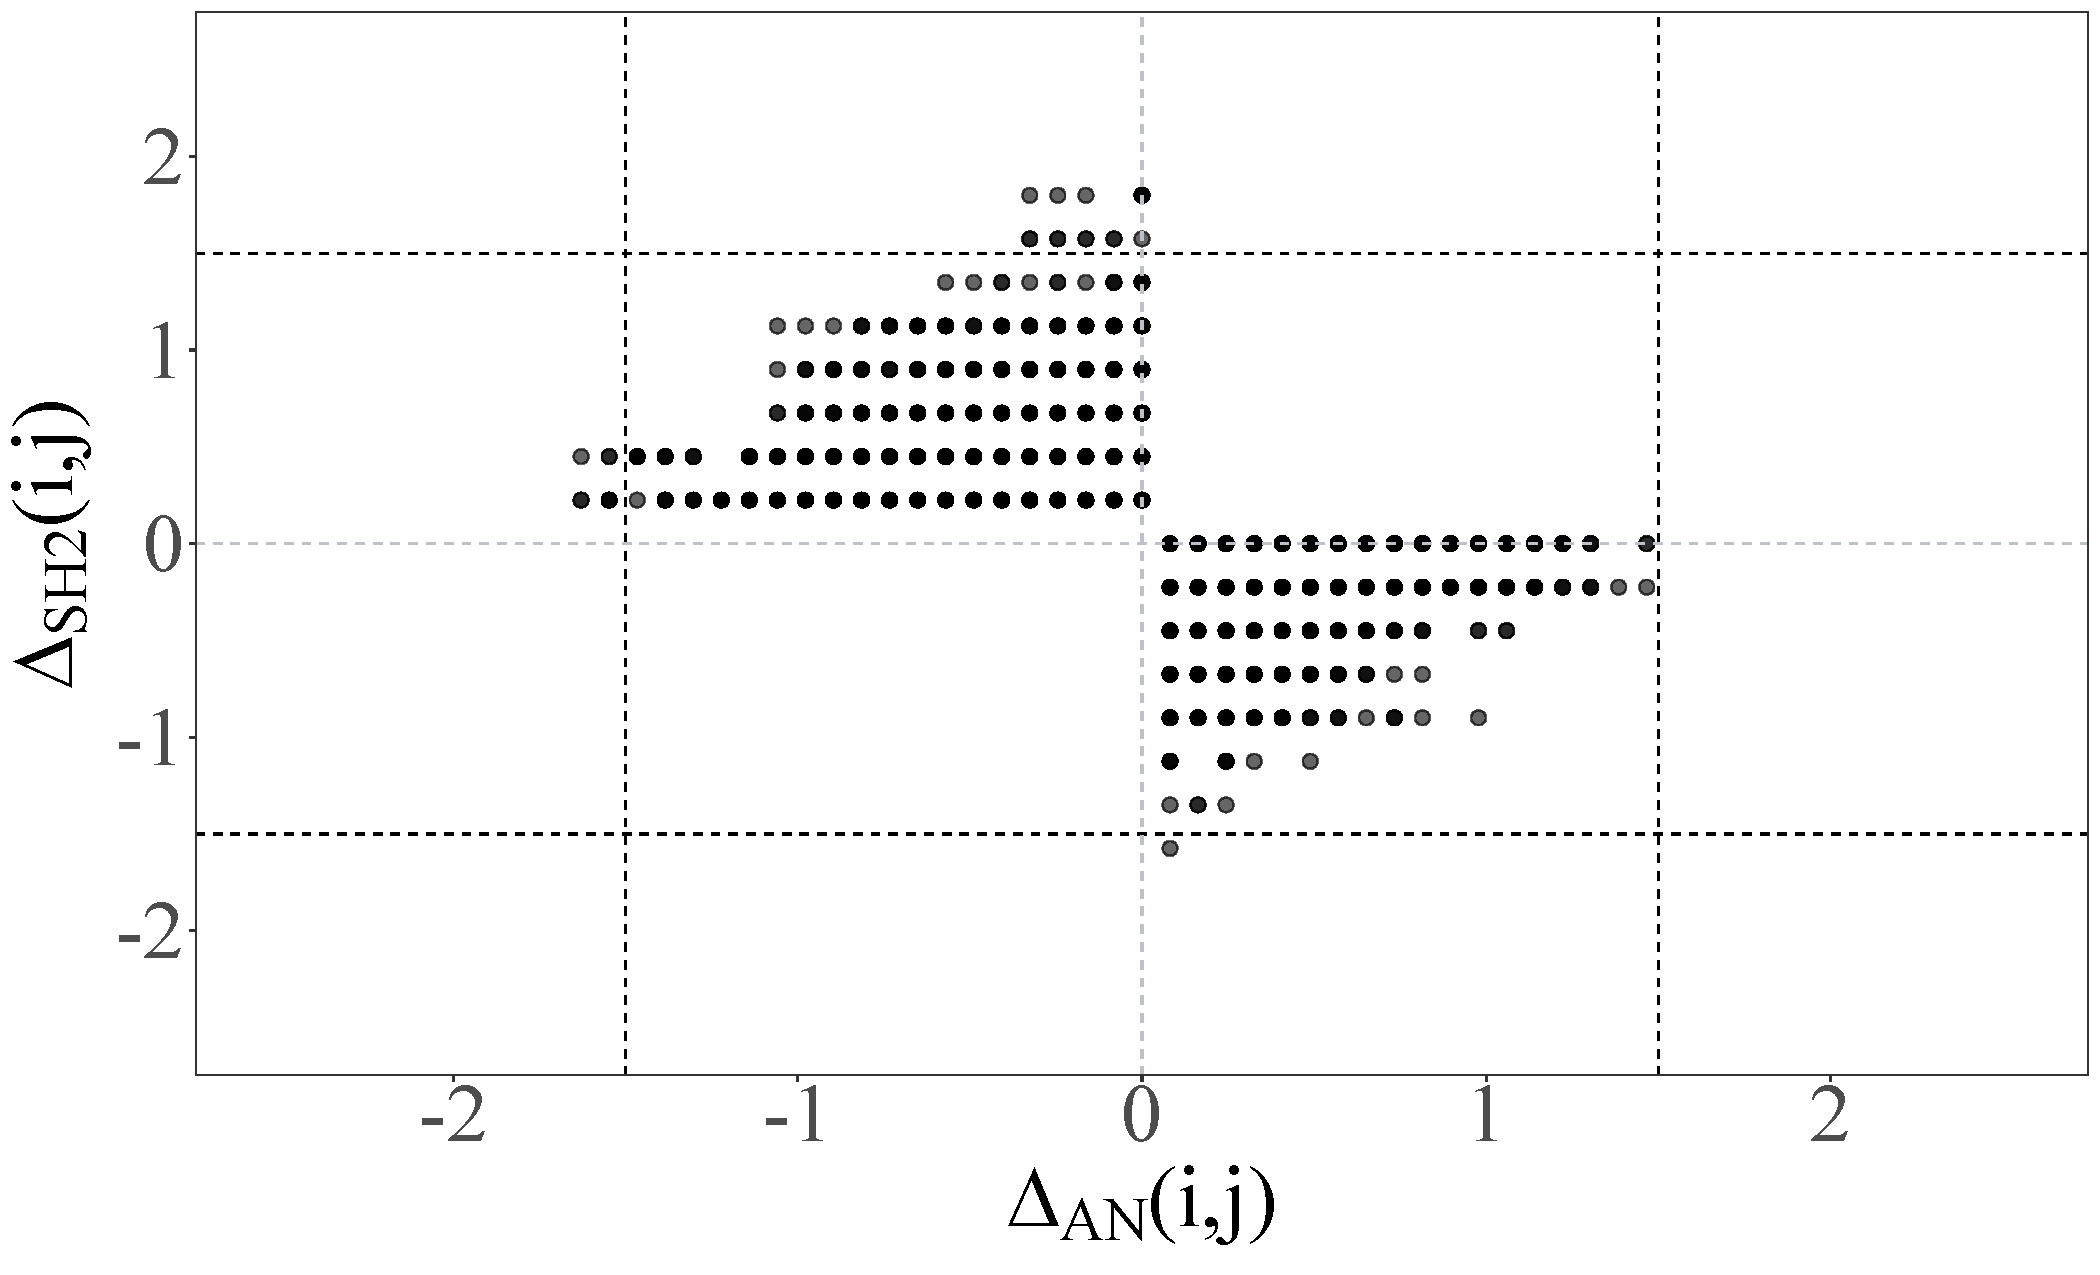
\includegraphics[width=\linewidth]{img/butterfly-AN-SH2}
 				\onslide<2>
                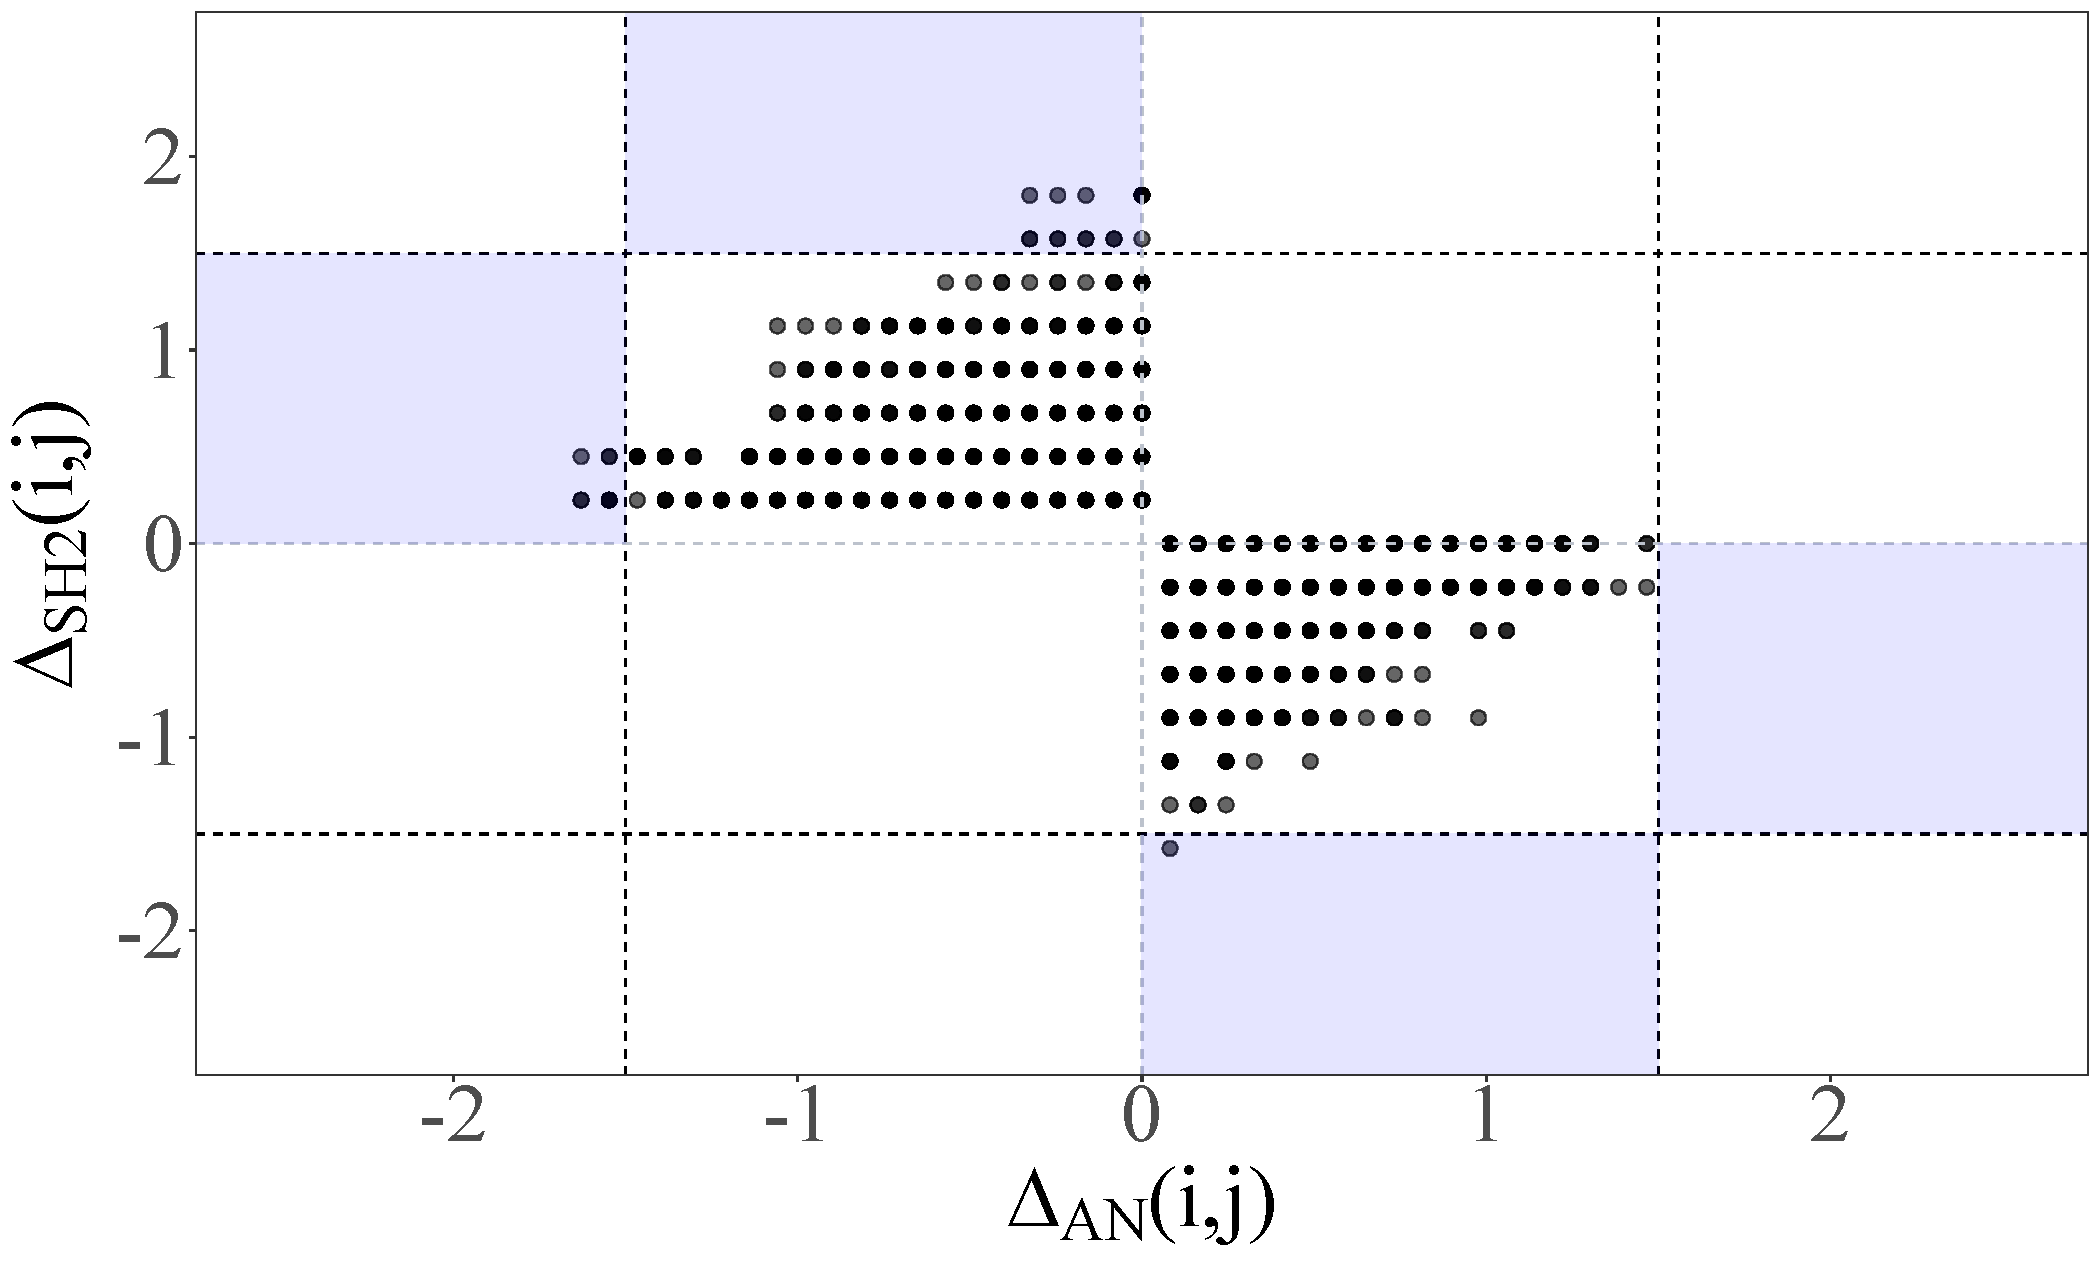
\includegraphics[width=\linewidth]{img/butterfly-AN-SH2-01}
 			\end{overprint}

 		\end{column}
 		\begin{column}{.50\linewidth}
 			\begin{overprint}
	\onslide<1>
	\centering
	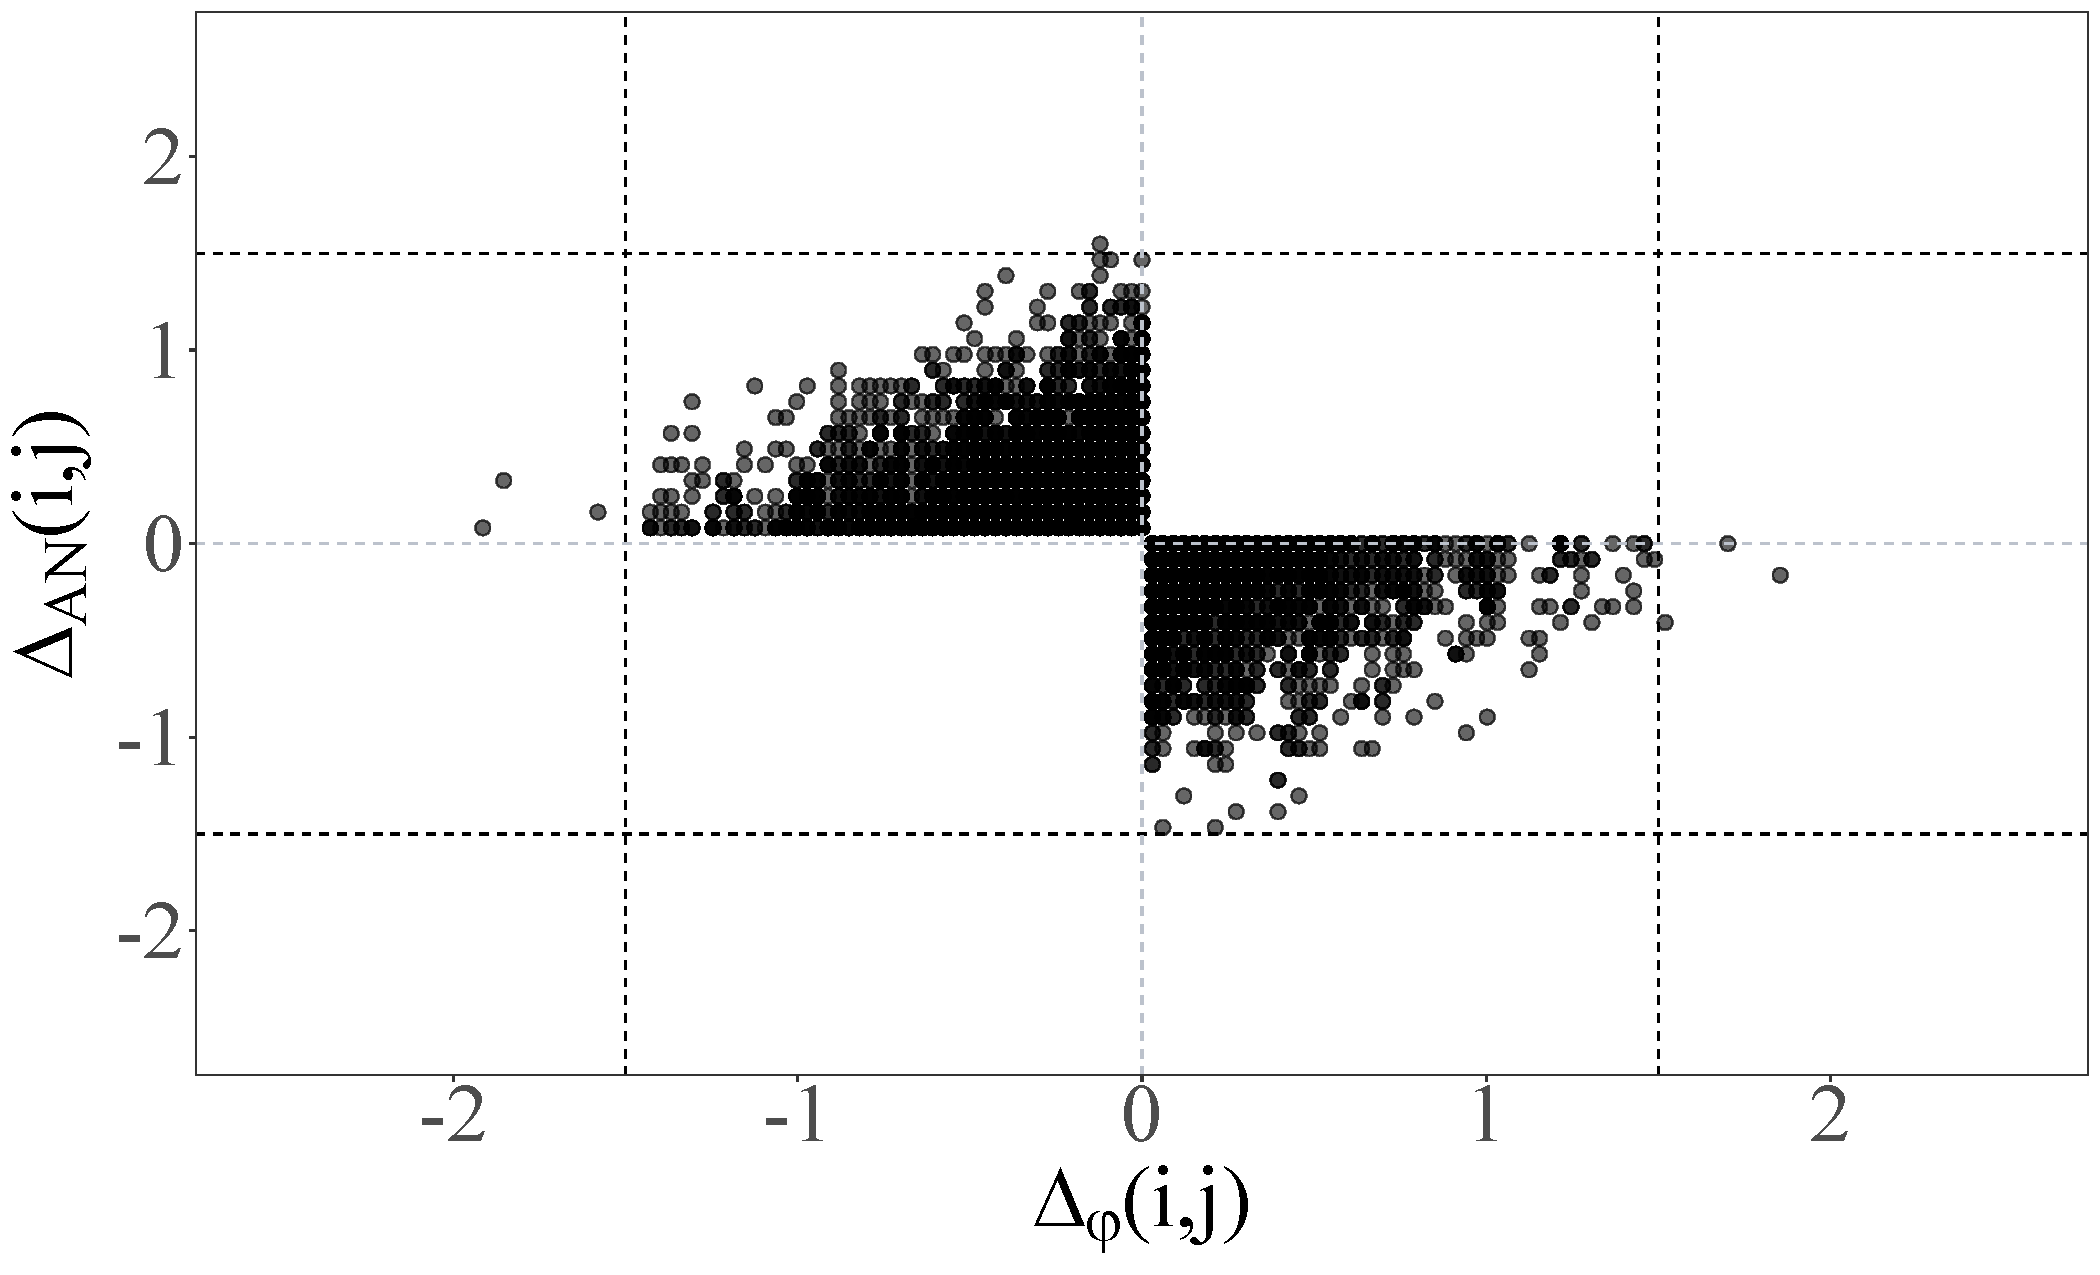
\includegraphics[width=\linewidth]{img/butterfly-PHI-AN}
	\onslide<2>
	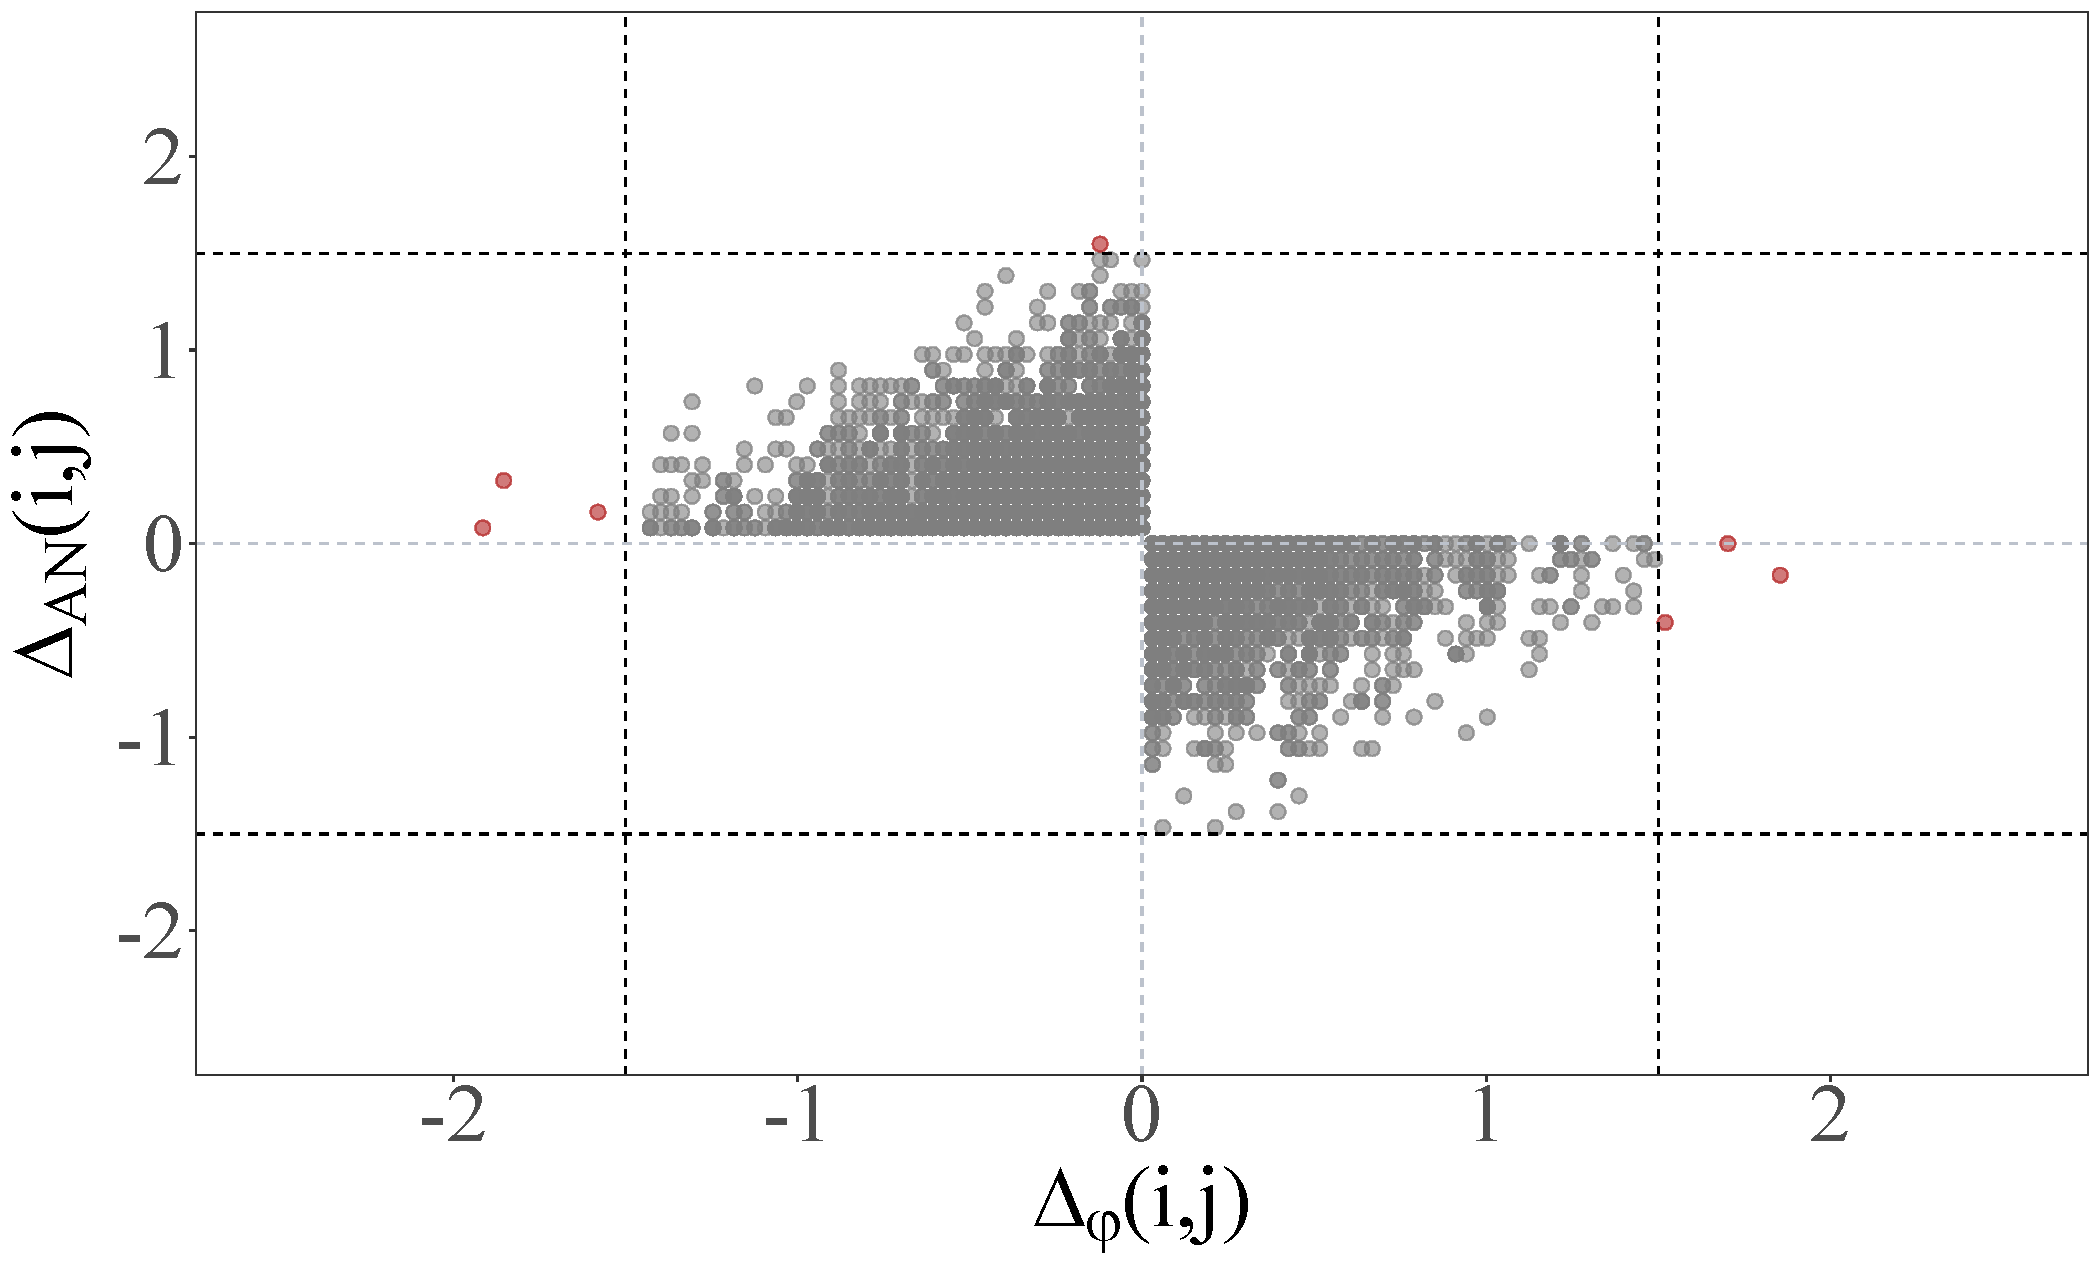
\includegraphics[width=\linewidth]{img/butterfly-PHI-AN-01}
\end{overprint}
 		\end{column}
 	\end{columns}
 	
 	
 \end{frame}
 




 
 \subsection{Results: Group differences}
 
 \begin{frame}{Attempt-based SM}
\begin{table}	
	\centering
	\begin{tabular}{ l r r r r}
		
		\hline
		&	\multicolumn{1}{c}{KR}	&	\multicolumn{1}{c}{SH1}	&	\multicolumn{1}{c}{P1}	&	\multicolumn{1}{c}{P1'}		\\
		
		&	\multicolumn{1}{c}{\color{black!40}\emph{d}}	&	\multicolumn{1}{c}{\color{black!40}\emph{d}}	&	\multicolumn{1}{c}{\color{black!40}\emph{d}}	&	\multicolumn{1}{c}{\color{black!40}\emph{d}} 		\\\hline 

	Gender	&	1.84\phantom{\sym{***}}	&	$2.11\sym{*}$\phantom{\sym{**}}	& \cellcolor<5-5>{red!70}	1.69\phantom{\sym{***}}	&	2.03\sym{*}\phantom{\sym{**}}	\\
&	\color{black!40}0.19\phantom{\sym{***}}	&	\color{black!40}0.21\phantom{\sym{***}}	&	\color{black!40}0.17\phantom{\sym{***}}	&	\color{black!40}0.20\phantom{\sym{***}}	\\
\cellcolor<2-2>{green!20}	Test order	& \cellcolor<3-3>{red!70}	$-0.15$\phantom{\sym{***}}	&	0.80\phantom{\sym{***}}	& \cellcolor<3-3>{white} \cellcolor<4-4>{red!70}	$-0.48$\phantom{\sym{***}}	&	0.28\phantom{\sym{***}}	\\
&	\color{black!40}$-0.01$\phantom{\sym{***}}	&	\color{black!40}0.08\phantom{\sym{***}}	&	\color{black!40}$-0.05$\phantom{\sym{***}}	&	\color{black!40}0.03\phantom{\sym{***}}	\\
Adm. Modality	&	$-2.85\sym{**}$\phantom{\sym{*}}	&	$-1.93$\phantom{\sym{***}}	&	$-2.69\sym{**}$\phantom{\sym{*}}	&	$-2.35\sym{*}$\phantom{\sym{**}}	\\
&	\color{black!40}$-0.29$\phantom{\sym{***}}	&	\color{black!40}$-0.19$\phantom{\sym{***}}	&	\color{black!40}$-0.27$\phantom{\sym{***}}	&	\color{black!40}$-0.24$\phantom{\sym{***}}	\\
\cellcolor<2-2>{green!20}Schooling	&	3.95$\sym{***}$	&	$3.56\sym{***}$	&	3.82$\sym{***}$	&	$3.85\sym{***}$	\\
&	\color{black!40}0.39\phantom{\sym{***}}	&	\color{black!40}0.36\phantom{\sym{***}}	&	\color{black!40}0.38\phantom{\sym{***}}	&	\color{black!40}0.39\phantom{\sym{***}}	\\
		\hline
	\end{tabular}
\end{table}
 \end{frame}
 

  \begin{frame}{Latency-based SM}
 	\begin{table}	
 		\centering
 		\begin{tabular}{ l rrr}
 			
 			\hline
 			&	\multicolumn{1}{c}{SH2}	&	\multicolumn{1}{c}{AN}	&	\multicolumn{1}{c}{T}	\\
 			
 				&	\multicolumn{1}{c}{\color{black!40}\emph{d}}	&	\multicolumn{1}{c}{\color{black!40}\emph{d}}	&	\multicolumn{1}{c}{\color{black!40}\emph{d}} \\ \hline 
 			
Gender	&	1.64\phantom{\sym{***}}	& \cellcolor<3-3>{red!70}	1.88\phantom{\sym{***}}	&	2.10\sym{*}\phantom{\sym{**}}		\\
&	\color{black!40}0.17\phantom{\sym{***}}	&	\color{black!40}0.19\phantom{\sym{***}}	&	\color{black!40}0.21\phantom{\sym{***}}	\\
\cellcolor<2-2>{green!20}Test order	&	0.37\phantom{\sym{***}}	&	0.99\phantom{\sym{***}}	&	0.95\phantom{\sym{***}}	\\
&	\color{black!40}0.04\phantom{\sym{***}}	&	\color{black!40}0.10\phantom{\sym{***}}	&	\color{black!40}0.10\phantom{\sym{***}}	\\
\cellcolor<2-2>{green!20}Adm. Order	&	$-2.90$\sym{**}\phantom{\sym{*}}	&	$-2.33$\sym{*}\phantom{\sym{**}}	&	$-2.84$\sym{**}\phantom{\sym{*}}	\\
&	\color{black!40}$-0.29$\phantom{\sym{***}}	&	\color{black!40}$-0.23$\phantom{\sym{***}}	&	\color{black!40}$-0.29$\phantom{\sym{***}}	\\
\cellcolor<2-2>{green!20}Schooling	&	5.52\sym{***}	&	5.32\sym{***}	&	5.13\sym{***}	\\
&	\color{black!40}0.56\phantom{\sym{***}}	&	\color{black!40}0.54\phantom{\sym{***}}	&	\color{black!40}0.52\phantom{\sym{***}}	\\
 			\hline
 		\end{tabular}
 	\end{table}
 \end{frame}
 
 \section{Food for thoughts}
 
 \begin{frame}
% 	    \begin{tikzpicture}[remember picture, overlay]
% 		\node[anchor=north east, yshift=-3.5] at (current page.north east) {
% 			
\includegraphics[width=0.1\textwidth]{img/food00}
% 		};
% 	\end{tikzpicture}


  \begin{tikzpicture}[remember picture, overlay]
	% Place the image
	\node[anchor=center] at (current page.center) {
		
\includegraphics[width=0.8\textwidth]{img/sum-scores} % Replace with your image file
	};
	
		\node[anchor=north, yshift=3cm] at (current page.center) {
		\textcolor{unipd}{\Large\textbf{Are we sure sum scores are a good idea...?}}
	};

	\node[anchor=south west, rotate=45, xshift=4cm, yshift=-3cm] at (current page.center) {
		\textcolor{unipd}{\Huge\textbf{??}}
	};
	\node[anchor=north east, xshift=-3cm, yshift=-1cm] at (current page.center) {
		\textcolor{unipd}{\Huge\textbf{???}}
	};
	\node[anchor=north west, xshift=3cm, yshift=-2cm] at (current page.center) {
		\textcolor{unipd}{\Huge\textbf{??}}
	};
	
	\onslide<2->
		\node[anchor=south, yshift=-3.5cm] at (current page.center) {
		\textcolor{unipd}{\textbf{Sum scores of ordinal data bring to a multiverse of contrasting results}}
	};
\end{tikzpicture}

%Punteggi somma su dati ordinali non va bene, porta a un multiverso di risultati contrastanti
 
 %		\vfill
 %	\scriptsize
 %	Research founded by the project ``Computerized, Adaptive and Personalized Assessment of Executive Functions and Fluid Intelligence''
 %	(PRIN 2020, Prot. 20209WKCLL, P.I. Prof. Luca Stefanutti)
 \end{frame}
 
 
 \begin{frame}
 
 	\begin{figure}
 		\centering
 		\includegraphics[width=.5\linewidth]{img/iceberg}
 	\end{figure}
 \end{frame}
 
 \begin{frame}
 		\vspace*{-10mm}
 	\begin{figure}
 		\centering
 	
\includegraphics[width=.15\linewidth]{img/food00}
 	\end{figure}
 	
 	Sum scores of ordinal data bring to a multiverse of contrasting results 
 	
 	\vspace{1.5mm}
 	Increasing the number of items does not solve the issue.... it worsens it!
 	
 		\vspace{1.5mm}
 		Meaningfulness of psychological measures and reproducibility are interlaced
 	
 	\onslide<2->
 	\begin{block}{Bright side:}
 		
 		Sum scores of truly dichotomous data (i.e., true vs. false, correct vs. incorrect) are meaningful 
 	\end{block}
 	
 	\onslide<1->
 	\vfill
 	\scriptsize
 	Research founded by the project ``Computerized, Adaptive and Personalized Assessment of Executive Functions and Fluid Intelligence''
 	(PRIN 2020, Prot. 20209WKCLL, P.I. Prof. Luca Stefanutti)
 \end{frame}
 
 
\end{document}